\chapter{Synthesis: Unifying Temporal Dynamics and Spatial Topology}
\label{chap:synthesis}

\section{Introduction}
\label{sec:ch7_intro}

The final question is whether the temporal characterization (Chapter~\ref{chap:dynamics}) and the spatial characterization (Chapter~\ref{chap:arspi_net}) correspond to the same underlying structure or whether they measure independent aspects of the signal---a test of cross-scale correspondence between local reservoir dynamics and global network topology.

The preceding chapters established two distinct characterization axes for affective EEG processing in ARSPI-Net. Chapter~\ref{chap:dynamics} developed the dynamical axis, extracting per-electrode temporal descriptors from the reservoir's internal state evolution and demonstrating that these descriptors are condition-sensitive (all seven metrics distinguish emotional from non-emotional input) but not strongly clinically sensitive at the channel-averaged level. Chapter~\ref{chap:arspi_net} developed the spatial axis by treating electrodes as nodes in a functional connectivity graph, characterizing propagation regimes and topological clinical phenotypes, and demonstrating that the graph topology carries the strongest clinical signals (SUD $p = 0.0004$). Each axis accesses different information: the temporal axis encodes what stimulus is being processed, while the spatial axis encodes whose brain is processing it.

The present chapter asks whether these two axes are aligned. In the fMRI structure--function coupling literature, alignment between local functional properties and global topological role is a hallmark of organized neural processing \cite{Deco2015,honey_network_2007,suarez_linking_2020}. If an electrode that occupies a central position in the functional graph also produces a distinctive reservoir trajectory, then the temporal and spatial characterizations are coupled views of a single underlying signal organization rather than independent descriptions. If they are not aligned, the two axes access genuinely different layers of the EEG. Both outcomes are informative: coupling reveals systems-level coordination, while independence reveals that the multi-axis instrument captures non-redundant structure. Critically, the coupling measure $\kappa$ is itself an intrinsically interpretable quantity: it tells a clinician whether a patient's temporal dynamics and spatial topology \emph{agree or disagree} at each electrode---a systems-level characterization of neural organization that no single-stage classifier can provide.

The chapter presents five experiments at four-class resolution (Threat, Mutilation, Cute, Erotic), which provides within-valence subcategory contrasts inaccessible at three-class. Section~\ref{sec:ch7_3class} then replicates the core findings at three-class resolution (Negative, Neutral, Pleasant), where the $3.6\times$ stronger condition signal provides tighter statistical confidence. The cross-granularity comparison reveals which coupling properties are robust and which are regime-dependent.

Five experiments are organized in a deductive chain. Experiment~7.1 tests whether coupling exists above permutation-null baselines. Experiment~7.2 decomposes the variance of coupling strength into subject and category components. Experiment~7.3 examines whether the structure of coupling differs across within-valence affective subcategories. Experiment~7.4 tests whether diagnosis-associated groups differ in coupling strength. Experiment~7.5 asks whether the two descriptor families carry complementary discriminative information for clinical detection.


\section{Mathematical Framework}
\label{sec:ch7_framework}

\subsection{Data Objects}

For each subject $s \in \{1,\ldots,211\}$ and category $c \in \{\text{Threat, Mutilation, Cute, Erotic}\}$, two per-electrode descriptor matrices are constructed from the same $1229 \times 34$ category-level trial-averaged EEG epoch.

The \textbf{dynamical profile matrix} $\mathbf{D}_{s,c} \in \mathbb{R}^{34 \times 7}$ contains the seven dual-gate validated metrics from Chapter~\ref{chap:dynamics} for each of the $N_c = 34$ electrodes: total spikes, mean firing rate, rate entropy, rate variance, temporal sparsity, permutation entropy~$\hat{H}_\pi$, and autocorrelation decay~$\tau_{AC}$. Each column of $\mathbf{D}_{s,c}$ is obtained by driving the validated reservoir ($N_{res}=256$, $\beta=0.05$, $M_{th}=0.5$, seed~42) with the z-scored single-channel EEG and extracting the metric from the resulting spike train and membrane potential trajectory.

The \textbf{topological profile matrix} $\mathbf{T}_{s,c} \in \mathbb{R}^{34 \times 2}$ contains two primary graph metrics for each electrode: weighted node strength and weighted clustering coefficient (Onnela formula) \cite{onnela_intensity_2005}. These are extracted from a $34 \times 34$ theta-band ($4$--$8$~Hz) time-averaged phase concentration (tPLV) matrix \cite{lachaux_measuring_1999}. Because the available data are category-level trial averages (one epoch per subject per category), the tPLV is computed as within-epoch phase concentration,
\begin{equation}
\label{eq:tplv}
\text{tPLV}_{ij} = \left|\frac{1}{T}\sum_{t=1}^{T} e^{j(\phi_i(t) - \phi_j(t))}\right|,
\end{equation}
where $\phi_i(t)$ is the instantaneous phase of the theta-filtered signal at electrode~$i$. This is not classical trial-to-trial phase-locking; it quantifies the temporal concentration of instantaneous phase differences within a single epoch. Node strength and weighted clustering are selected as primary topological metrics because they are the most stable graph measures on 34-node dense graphs \cite{rubinov_complex_2010}. Betweenness centrality and local efficiency are omitted from the primary analysis due to known instability at this graph density and node count.

\subsection{Coupling Measures}

The within-subject coupling matrix is defined by electrode-wise Spearman rank correlations between the two descriptor families:
\begin{equation}
\label{eq:coupling_C}
\mathbf{C}_{s,c} \in \mathbb{R}^{7 \times 2}, \quad (\mathbf{C}_{s,c})_{jk} = \rho_S(\mathbf{D}_{s,c}[:,j],\;\mathbf{T}_{s,c}[:,k]),
\end{equation}
where $\rho_S$ denotes Spearman correlation computed across the 34 electrodes. Each entry of $\mathbf{C}_{s,c}$ quantifies how one dynamical metric covaries with one topological metric across the electrode array for a specific subject and category.

The scalar coupling strength is the normalized Frobenius norm:
\begin{equation}
\label{eq:kappa}
\kappa_{s,c} = \frac{\|\mathbf{C}_{s,c}\|_F}{\sqrt{p \cdot q}} = \frac{1}{\sqrt{14}}\sqrt{\sum_{j=1}^{7}\sum_{k=1}^{2}(\mathbf{C}_{s,c})_{jk}^2}.
\end{equation}
This normalization maps $\kappa$ to $[0,1]$ and enables comparison across configurations with different $p$ and $q$. A $\kappa$ near zero indicates that the dynamical and topological descriptor families are unaligned across electrodes; a $\kappa$ near one indicates that every dynamical metric is strongly rank-correlated with every topological metric.

Spearman $\mathbf{C}_{s,c}$ and scalar $\kappa_{s,c}$ are the primary coupling instruments throughout this chapter. Canonical Correlation Analysis (CCA) is available as a secondary multivariate summary but is not used for primary inference due to the modest ratio of electrodes ($N_c = 34$) to variables ($p + q = 9$), which produces upward-biased canonical correlations in small samples \cite{wang_cca_2020}.

\subsection{Null Model}

The electrode-permutation null shuffles the row indices of $\mathbf{T}_{s,c}$ relative to $\mathbf{D}_{s,c}$, breaking the electrode correspondence while preserving the marginal distributions of both descriptor families. For each of 2,000 permutations~$\pi$, a null coupling $\kappa_{s,c}^{(\pi)}$ is computed. The per-observation $p$-value is
\begin{equation}
p_{s,c} = \frac{1 + \#\{\kappa_{s,c}^{(\pi)} \ge \kappa_{s,c}\}}{1 + 2000}.
\end{equation}


\section{Data and Experimental Protocol}
\label{sec:ch7_protocol}

All experiments use the SHAPE Community dataset: $N = 211$ subjects (excluding subject~127), four IAPS subcategories (Threat, Mutilation, Cute, Erotic), yielding 844 subject--category observations. Each observation is a $1229 \times 34$ category-level trial-averaged EEG epoch at 1024~Hz, consistent with the data format in Chapters~\ref{chap:dynamics} and~5.

For each observation, the reservoir processes all 34 channels independently (28,696 total reservoir runs across the dataset). The tPLV matrix is computed from the same 34-channel epoch via theta-band filtering (3rd-order Butterworth, $4$--$8$~Hz) and Hilbert-transform phase extraction. Clinical metadata from the SHAPE psychopathology battery provides transdiagnostic diagnostic status for 206 of 211 subjects (5 missing), with mean comorbidity of 2.0 diagnoses per subject and 22 strict healthy controls (zero of five primary diagnoses: MDD, PTSD, SUD, GAD, ADHD). Note: this comorbidity count uses only the five primary diagnoses analyzed in this chapter; Chapter~\ref{chap:arspi_net} reports mean comorbidity of 2.8 using the full diagnostic panel (including eating disorders, mania, PDD, and other conditions), yielding 27 healthy controls under the broader definition.

Statistical inference throughout uses nonparametric methods: Wilcoxon signed-rank for paired contrasts, Mann--Whitney~$U$ for group comparisons, and permutation tests for interaction effects. Multiple comparison correction uses Bonferroni within defined families.


\section{Experiment 7.1: Coupling Existence}
\label{sec:exp7_coupling}

\subsection{Mathematical Motivation}

Both $\mathbf{D}_{s,c}$ and $\mathbf{T}_{s,c}$ are derived from the same underlying EEG epoch through different transformations: the reservoir maps each channel's temporal signal into a dynamical descriptor, while the tPLV maps all pairwise phase relationships into a topological descriptor. If an electrode that participates in strong phase-locked interactions also drives the reservoir into a distinctive dynamical regime, then $\mathbf{D}_{s,c}$ and $\mathbf{T}_{s,c}$ will be rank-correlated across the electrode array. The observable quantities are the $7 \times 2$ coupling matrix $\mathbf{C}_{s,c}$, the scalar $\kappa_{s,c}$, and their distribution across 844 observations relative to the electrode-permutation null.

\subsection{Experimental Design}

For each of 844 observations, $\mathbf{C}_{s,c}$ and $\kappa_{s,c}$ are computed from $\mathbf{D}_{s,c}$ ($34 \times 7$) and $\mathbf{T}_{s,c}$ ($34 \times 2$). The electrode-permutation null generates 2,000 null $\kappa$ values per observation. Group-level inference aggregates all 844 observed $\kappa$ values against their corresponding null medians using a one-sided Wilcoxon signed-rank test ($\kappa_{\text{obs}} > \kappa_{\text{null}}$). Because the 844 observations contain four per subject (one per category), a confirmatory subject-level analysis averaging $\kappa$ across categories ($N = 211$ independent observations) was also conducted; the coupling effect remains significant ($p < 0.001$, one-sample Wilcoxon against zero), confirming that the result is not inflated by within-subject dependence.

\subsection{Raw Observation}

\begin{figure}[htbp]
\centering
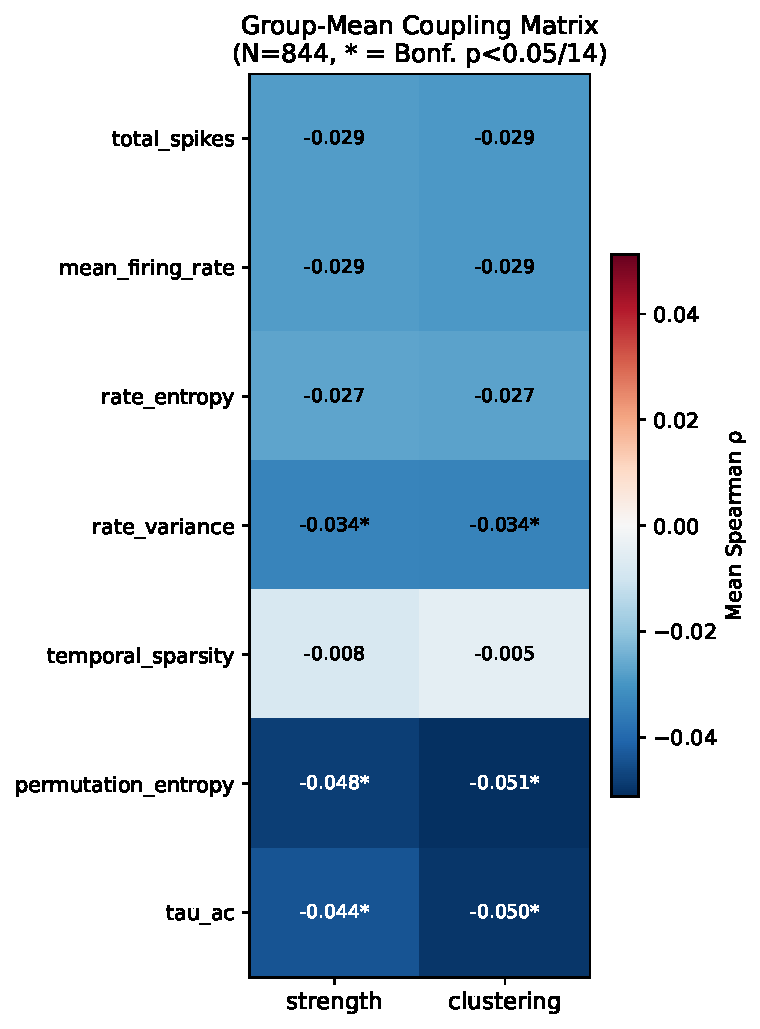
\includegraphics[width=0.65\textwidth]{pictures/chSynthesis/fig7_A1_mean_coupling_matrix.pdf}
\caption{Group-mean signed coupling matrix $\bar{\mathbf{C}}$ across all 844 observations ($N = 211$ subjects $\times$ 4 categories). Rows: seven dual-gate validated dynamical metrics. Columns: weighted strength and weighted clustering. All 14 entries are negative. Asterisks denote Bonferroni significance ($p < 0.05/14$). The four significant cells are rate variance, permutation entropy, and $\tau_{AC}$ paired with both topological metrics.}
\label{fig:mean_C}
\end{figure}

The group-mean coupling matrix (Figure~\ref{fig:mean_C}) reveals a striking and uniform pattern: all 14 dynamical-topological correlations are negative. Electrodes with higher connectivity strength and higher clustering produce reservoir trajectories with lower complexity, lower rate variance, and faster autocorrelation decay. The mean $\rho$ values range from $-0.005$ (temporal sparsity $\times$ clustering) to $-0.051$ (permutation entropy $\times$ clustering).

\begin{figure}[htbp]
\centering
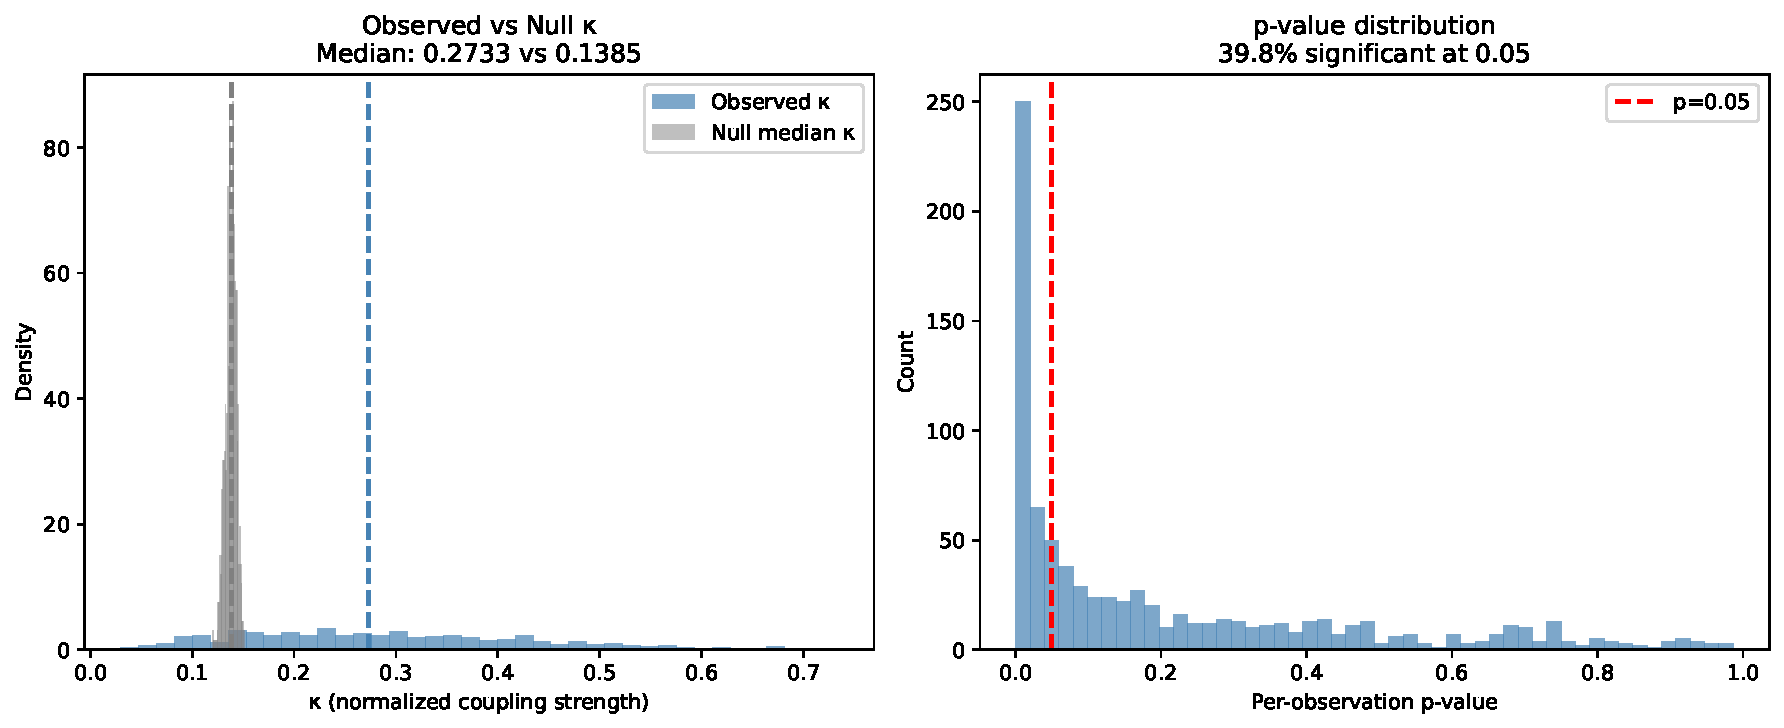
\includegraphics[width=0.95\textwidth]{pictures/chSynthesis/fig7_A2_kappa_vs_null.pdf}
\caption{Left: density distributions of observed $\kappa$ (median $= 0.273$) versus electrode-permutation null median $\kappa$ (median $= 0.139$). The observed distribution is shifted rightward, with negligible overlap. Right: per-observation $p$-value histogram. $39.8\%$ of observations reach $p < 0.05$; $23.6\%$ reach $p < 0.01$.}
\label{fig:kappa_null}
\end{figure}

Figure~\ref{fig:kappa_null} shows the distribution of $\kappa_{s,c}$ across all 844 observations alongside the null. The observed $\kappa$ distribution (median $= 0.273$, range $[0.030, 0.734]$) is displaced rightward from the null (median $= 0.139$). The $p$-value distribution shows a prominent spike near zero: $39.8\%$ of individual observations reach $p < 0.05$ against their own permutation null.

\begin{figure}[htbp]
\centering
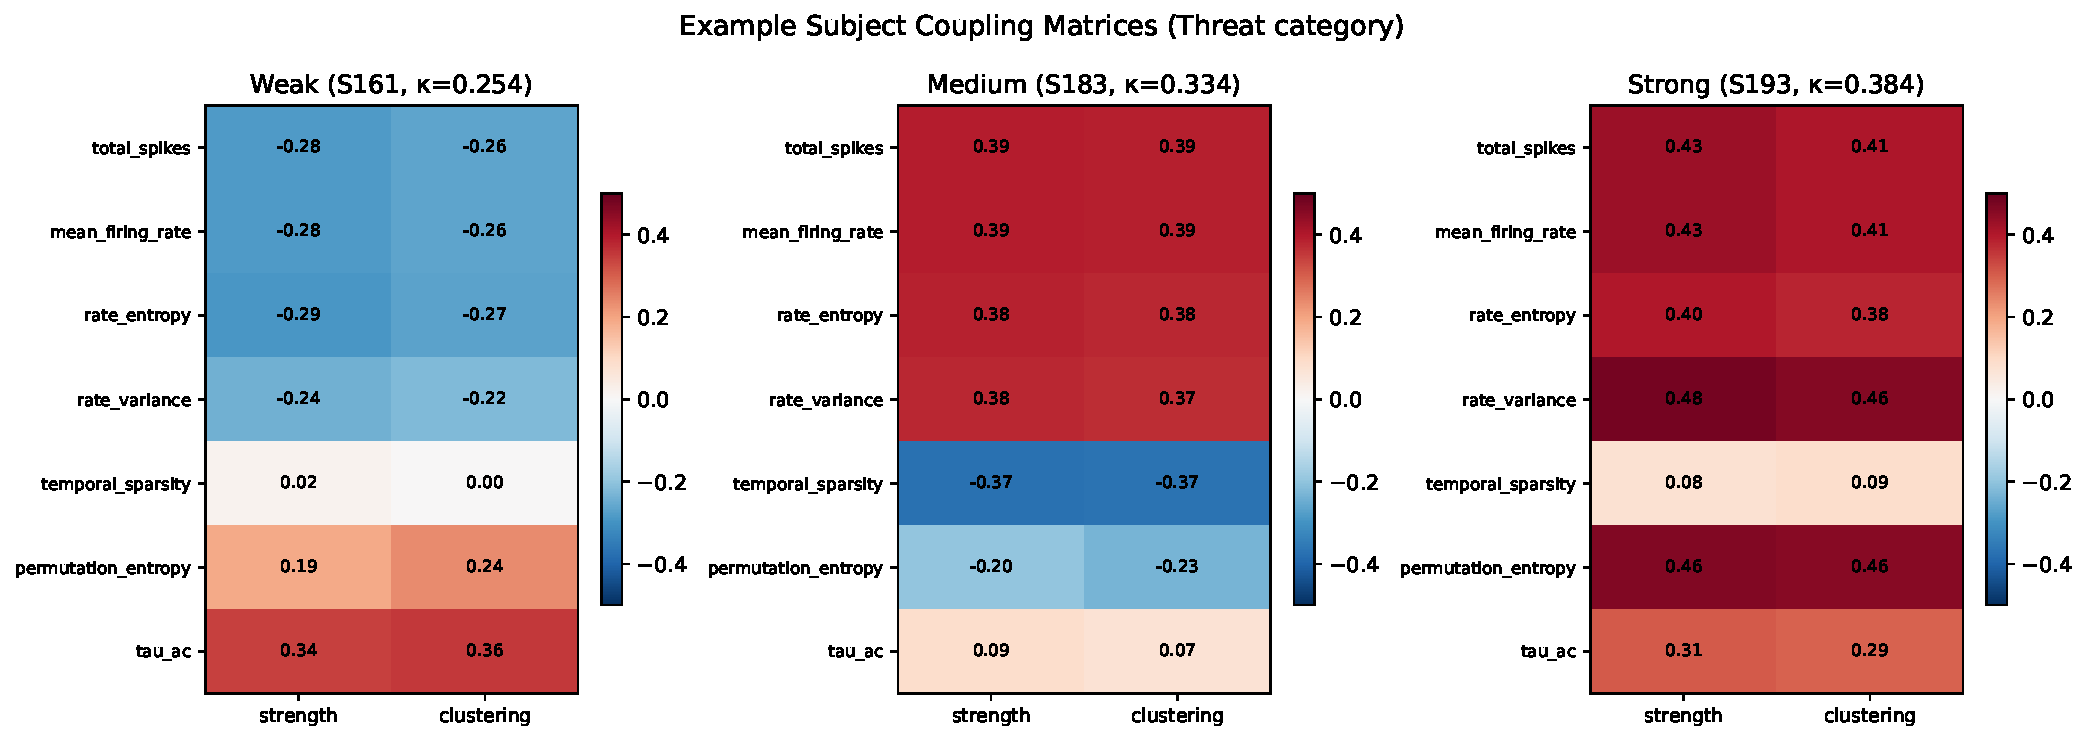
\includegraphics[width=0.95\textwidth]{pictures/chSynthesis/fig7_A3_example_subjects.pdf}
\caption{Example coupling matrices for three subjects (Threat category), selected at the 10th, 50th, and 90th percentiles of subject-mean $\kappa$. Individual-level coupling matrices show substantial inter-subject heterogeneity in both magnitude and sign pattern.}
\label{fig:example_subjects}
\end{figure}

Figure~\ref{fig:example_subjects} reveals substantial inter-subject heterogeneity. Subject~161 ($\kappa = 0.254$) shows negative spike-metric correlations but positive $\tau_{AC}$ correlations. Subject~183 ($\kappa = 0.334$) shows the opposite pattern. Subject~193 ($\kappa = 0.384$) shows uniformly positive correlations. The group-mean matrix is uniformly negative because negative-coupling subjects outnumber positive ones, but the population contains subjects with both coupling directions. The magnitudes within individual subjects ($|\rho| \approx 0.2$--$0.5$) are considerably larger than the group means ($|\rho| \approx 0.03$--$0.05$), indicating partial cancellation across subjects.

\subsection{Quantitative Analysis}

The group-level Wilcoxon signed-rank test on $\kappa_{\text{obs}} - \kappa_{\text{null median}}$ yields $W = 338{,}144$, $p = 4.98 \times 10^{-113}$, $d_z = 1.063$. Coupling between the dynamical and topological descriptor families exceeds the electrode-permutation null with an effect size exceeding one standard deviation of the paired difference distribution.

\begin{table}[htbp]
\centering
\caption{Coupling existence summary (Experiment~7.1).}
\label{tab:coupling_existence}
\small
\begin{tabular}{lcccc}
\toprule
\textbf{Statistic} & \textbf{Observed} & \textbf{Null median} & \textbf{$d_z$} & \textbf{$p$} \\
\midrule
Median $\kappa$ & 0.273 & 0.139 & 1.063 & $4.98 \times 10^{-113}$ \\
\% observations $p < 0.05$ & 39.8\% & 5.0\% (expected) & --- & --- \\
\% observations $p < 0.01$ & 23.6\% & 1.0\% (expected) & --- & --- \\
\bottomrule
\end{tabular}
\end{table}

Within the group-mean matrix, four of 14 cells reach Bonferroni significance ($p < 0.05/14 = 0.00357$): permutation entropy $\times$ clustering ($\rho = -0.051$, $p = 1.9 \times 10^{-6}$), $\tau_{AC} \times$ clustering ($\rho = -0.050$, $p = 3.5 \times 10^{-6}$), permutation entropy $\times$ strength ($\rho = -0.048$, $p = 1.1 \times 10^{-5}$), and $\tau_{AC} \times$ strength ($\rho = -0.044$, $p = 4.7 \times 10^{-5}$). The temporal-structure-tracking metrics identified in Chapter~\ref{chap:dynamics} Experiment~6.4---permutation entropy and $\tau_{AC}$---are the metrics most strongly aligned with graph topology.

\subsection{Signal-Processing Interpretation}

The uniformly negative coupling direction admits a coherent signal-processing interpretation. Electrodes with high tPLV strength and clustering receive inputs that are strongly phase-locked to their neighbors. Phase-locked inputs are, by definition, temporally correlated with the network's dominant oscillatory modes. When such a signal drives the reservoir, the effective input diversity is lower than for a weakly coupled electrode whose signal reflects more independent temporal structure. Lower input diversity produces a simpler driven trajectory: lower permutation entropy, faster autocorrelation decay, and lower rate variance. The reservoir is measuring input independence, and highly connected nodes have less of it.

This interpretation is consistent with the data processing inequality \cite{cover_elements_2006}: the reservoir preserves at most the information already present in the input. High-connectivity electrodes deliver inputs with less independent temporal content, and the reservoir faithfully reflects that reduced content as lower trajectory complexity.

The observation that coupling exists motivates a natural question: what drives the variation in $\kappa$ across the 844 observations? If subject identity dominates---as it does for the raw descriptor spaces in Chapter~5---then coupling is an individual characteristic. If category explains a meaningful fraction, then coupling is modulated by stimulus content.


\section{Experiment 7.2: Variance Decomposition of Coupling Strength}
\label{sec:exp7_variance}

\subsection{Mathematical Motivation}

Chapter~5 demonstrated that subject identity explains 62.6\% of embedding variance versus 8.7\% for affective condition. If the same dominance holds for $\kappa$, coupling is a stable individual trait. If the subject fraction is smaller, the coupling statistic accesses a different layer of signal organization than the raw descriptor spaces from which it is derived. The observable quantities are the variance fractions $V_{\text{subj}}$, $V_{\text{cat}}$, and $V_{\text{resid}}$ in the two-way decomposition $\kappa_{s,c} = \mu + \alpha_s + \beta_c + \varepsilon_{s,c}$.

\subsection{Experimental Design}

The 844 $\kappa_{s,c}$ values from Experiment~7.1 are decomposed into subject ($\alpha_s$, 211~levels), category ($\beta_c$, 4~levels), and residual ($\varepsilon_{s,c}$) sum-of-squares components. The category effect is tested by permuting category labels within each subject (5,000 permutations), preserving subject structure while testing whether category differences exceed exchangeability. The intraclass correlation ICC(3,1) \cite{shrout_intraclass_1979} quantifies within-subject consistency of $\kappa$ across the four categories.

\subsection{Raw Observation}

\begin{figure}[htbp]
\centering
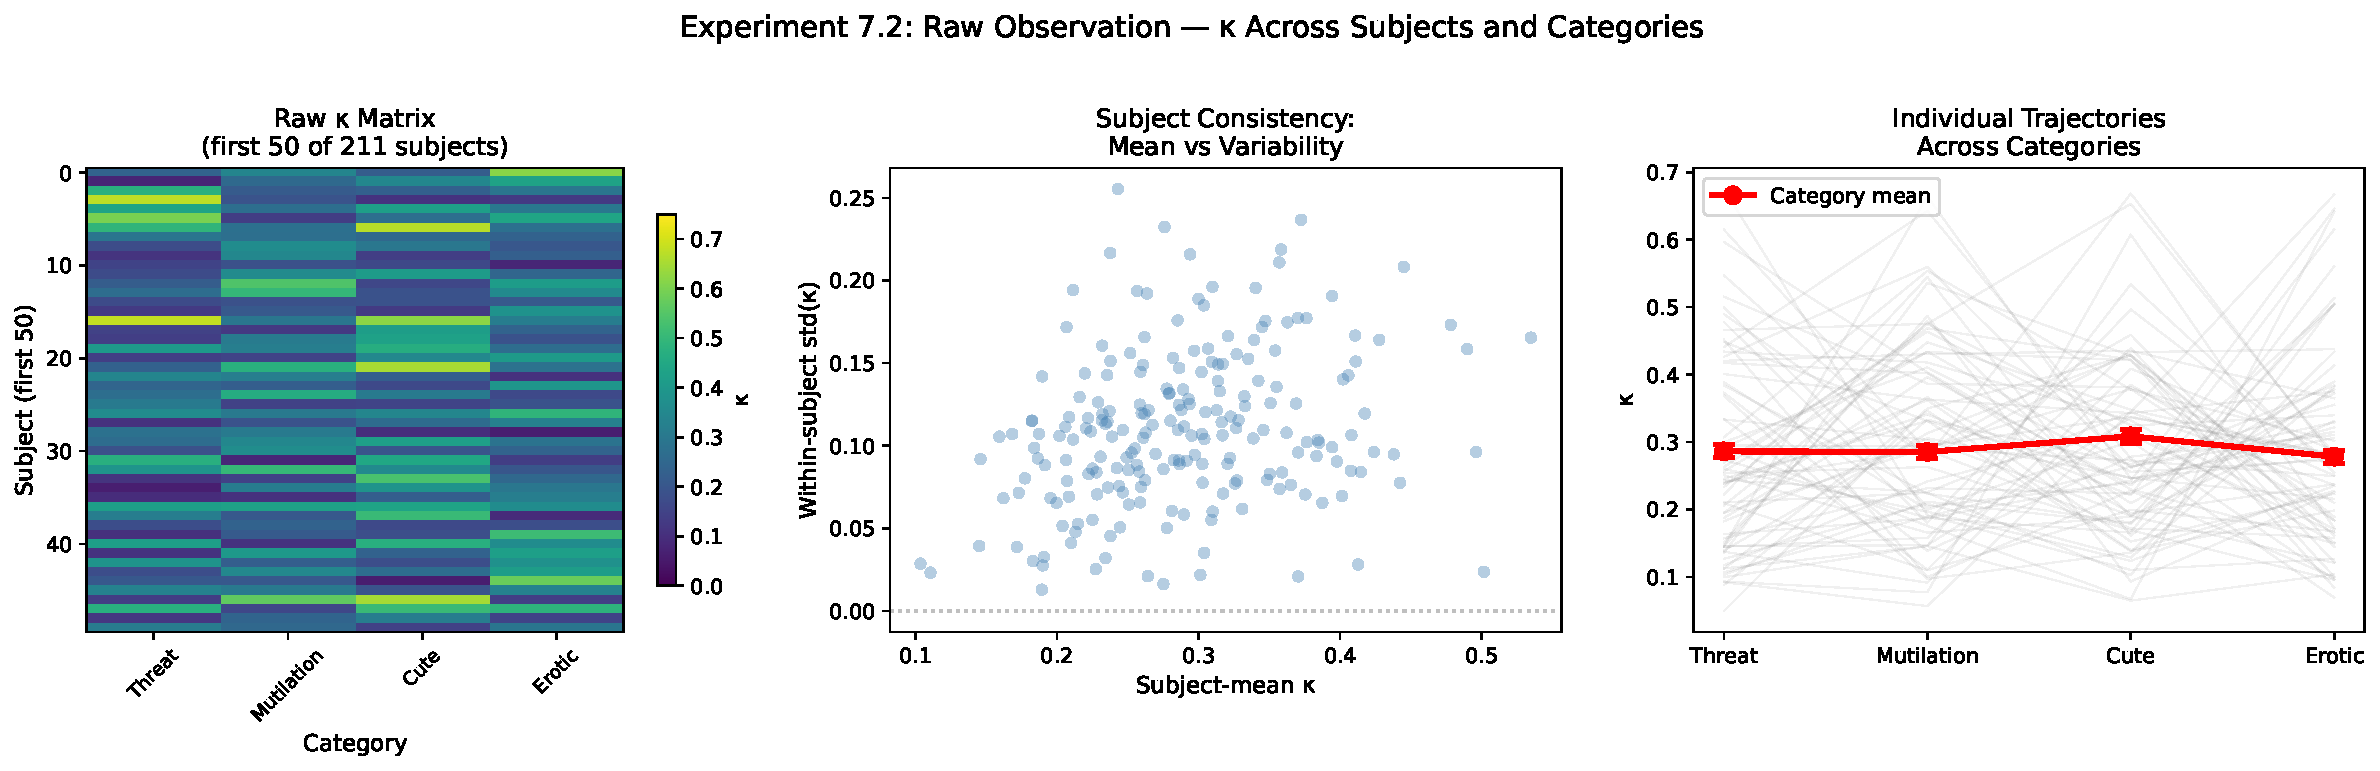
\includegraphics[width=0.95\textwidth]{pictures/chSynthesis/fig7_B1_raw_observation.pdf}
\caption{Raw observation of $\kappa$ across subjects and categories. Left: $\kappa$ matrix for the first 50 subjects (rows) $\times$ 4 categories (columns). Center: subject-mean $\kappa$ versus within-subject standard deviation. Right: individual subject trajectories across categories (gray) with category means (red). Within-subject variability (mean std $= 0.110$) exceeds between-subject variability (std of subject means $= 0.077$).}
\label{fig:raw_kappa_matrix}
\end{figure}

The category means span a narrow range: Cute ($\bar{\kappa} = 0.309$), Threat ($0.286$), Mutilation ($0.285$), Erotic ($0.278$). The between-category spread (max minus min mean) is 0.030. Within-subject standard deviation of $\kappa$ across the four categories averages 0.110---1.43 times the between-subject standard deviation of 0.077. The individual trajectories in Figure~\ref{fig:raw_kappa_matrix} show extensive crossing: a subject with high $\kappa$ under Threat may have low $\kappa$ under Cute, and vice versa.

\begin{figure}[htbp]
\centering
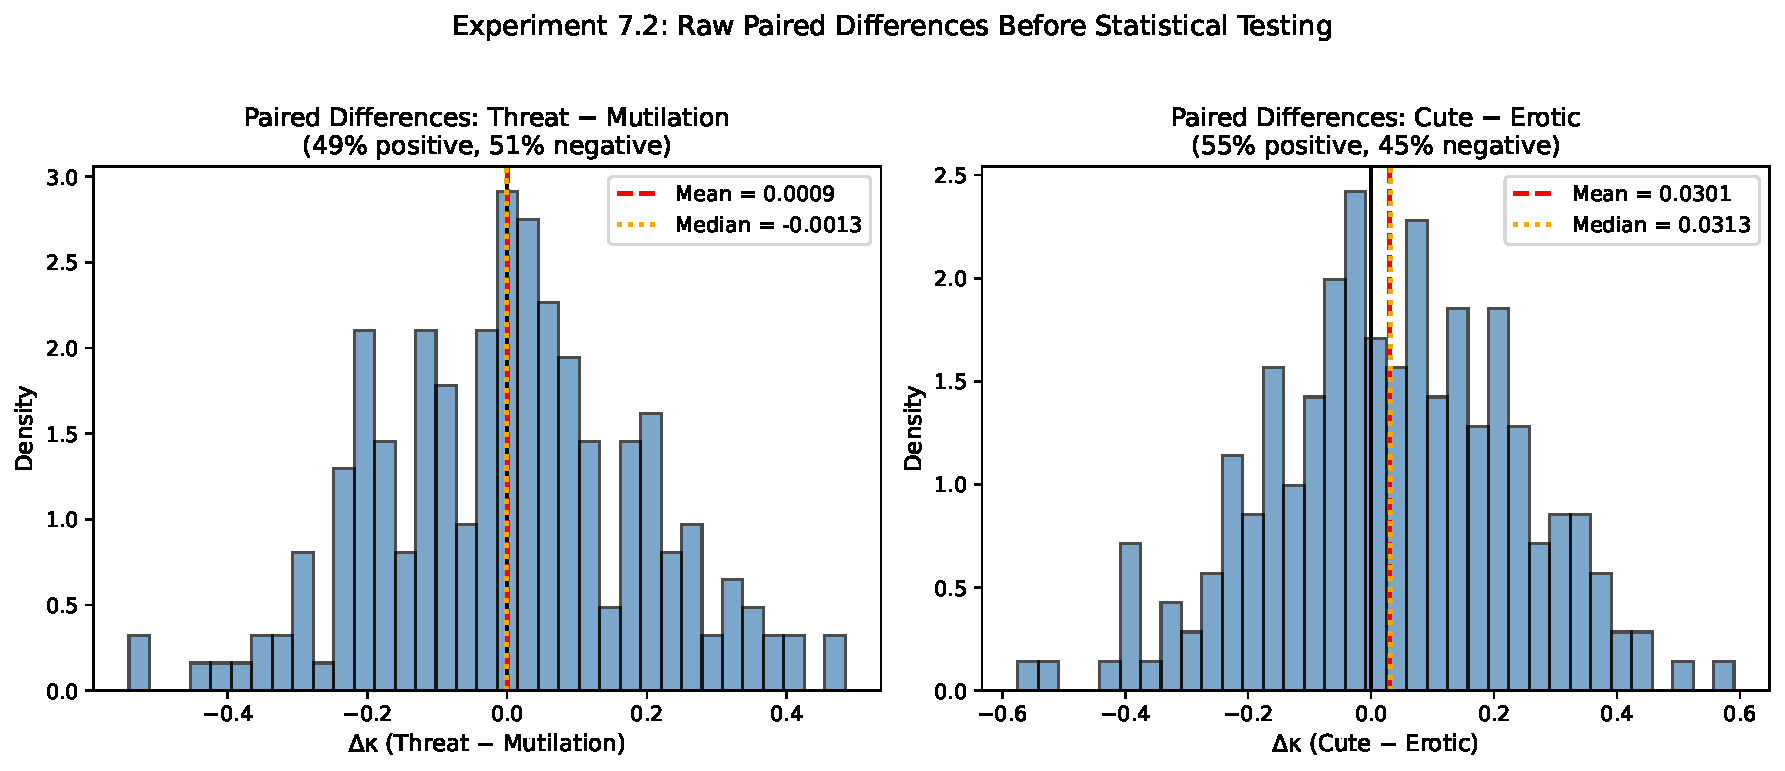
\includegraphics[width=0.95\textwidth]{pictures/chSynthesis/fig7_B2_raw_paired_differences.pdf}
\caption{Raw paired differences in $\kappa$ before statistical testing. Left: Threat $-$ Mutilation (centered on zero, 49.3\% positive). Right: Cute $-$ Erotic (shifted positive, 55.5\% positive, mean $\Delta\kappa = +0.030$).}
\label{fig:raw_paired_diff}
\end{figure}

The raw paired differences (Figure~\ref{fig:raw_paired_diff}) show that the Threat--Mutilation contrast is centered precisely on zero, while the Cute--Erotic contrast is shifted positive: Cute stimuli produce systematically higher coupling than Erotic stimuli.

\subsection{Quantitative Analysis}

\begin{figure}[htbp]
\centering
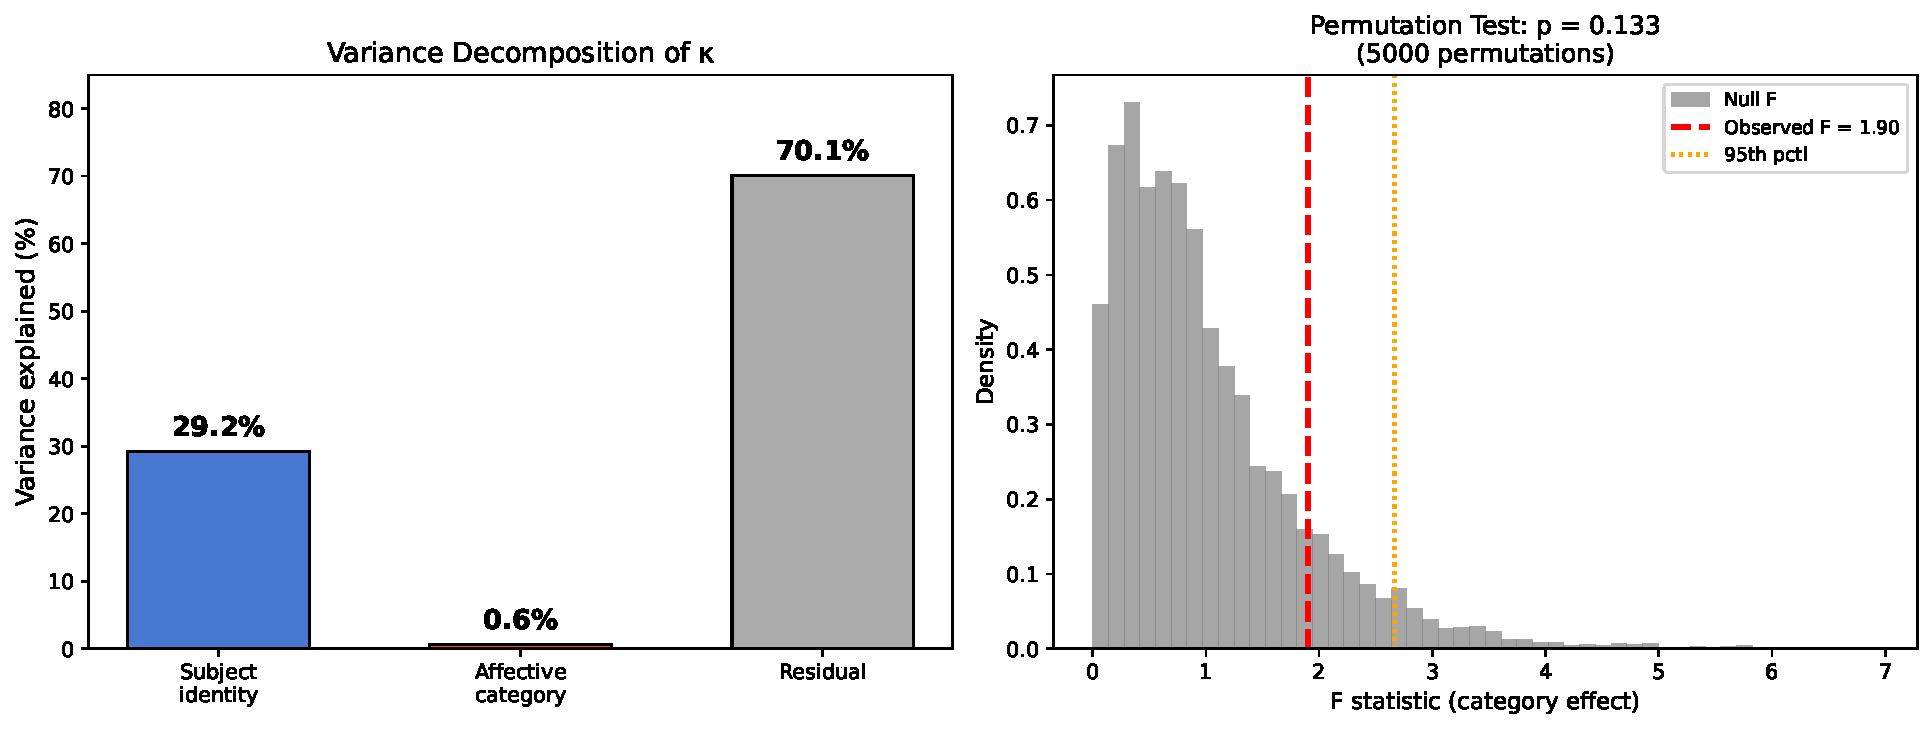
\includegraphics[width=0.95\textwidth]{pictures/chSynthesis/fig7_B3_variance_decomposition.pdf}
\caption{Left: variance decomposition of $\kappa$ into subject (29.2\%), category (0.6\%), and residual (70.1\%) components. Right: permutation null for the category $F$-statistic. The observed $F = 1.90$ falls below the 95th percentile of the null ($p = 0.133$).}
\label{fig:variance_decomp}
\end{figure}

\begin{table}[htbp]
\centering
\caption{Variance decomposition of $\kappa_{s,c}$ (Experiment~7.2).}
\label{tab:variance_decomp}
\small
\begin{tabular}{lcccc}
\toprule
\textbf{Component} & \textbf{\% Variance} & \textbf{$F$} & \textbf{$p$ (permutation)} \\
\midrule
Subject identity & 29.2\% & --- & --- \\
Affective category & 0.6\% & 1.90 & 0.133 \\
Residual & 70.1\% & --- & --- \\
\bottomrule
\end{tabular}
\end{table}

Subject identity explains 29.2\% of $\kappa$ variance, affective category explains 0.6\%, and the residual explains 70.1\% (Table~\ref{tab:variance_decomp}; Figure~\ref{fig:variance_decomp}). The category component does not reach significance by permutation test ($F = 1.90$, $p = 0.133$) or by Friedman test ($\chi^2 = 3.22$, $p = 0.359$). The ICC(3,1) of $\kappa$ across categories is 0.059, indicating that a subject's coupling strength in one category is essentially independent of their coupling in another.

The within-valence contrasts reveal a more specific pattern. Threat $-$ Mutilation shows no paired difference ($\Delta\kappa = -0.001$, $d_z = 0.005$, $p = 0.965$). Cute $-$ Erotic shows a small but significant difference ($\Delta\kappa = +0.031$, $d_z = 0.148$, $p = 0.025$), paralleling Chapter~\ref{chap:dynamics} Experiment~6.5's identification of Cute--Erotic as the strongest temporal-descriptor contrast.

\subsection{Interpretation and Significance}

Three observations are scientifically significant. First, the 29.2\% subject component is substantially smaller than the 62.6\% subject dominance observed in Chapter~5's embedding variance decomposition. Coupling is less subject-determined than the raw feature spaces from which it is derived. The coupling statistic strips away a substantial portion of individual-difference structure and exposes a quantity that is more observation-specific.

Second, the ICC of 0.059 indicates that coupling is not a stable individual trait. Each (subject, category) observation produces a coupling configuration that is largely independent of the same subject's coupling under a different stimulus. The raw features tell you mostly \emph{who} you are looking at; the coupling tells you mostly \emph{what is being processed}.

Third, the residual dominance (70.1\%) represents genuine within-subject, within-category variability in the temporal--spatial alignment. This variability is the reservoir's response to observation-specific properties of the driven EEG that are not captured by subject identity or broad category labels.

The Cute--Erotic $\kappa$ difference raises a natural question: when coupling strength increases for Cute relative to Erotic, which specific dynamical-topological relationships are driving the change?


\section{Experiment 7.3: Category-Conditioned Coupling Structure}
\label{sec:exp7_category}

\subsection{Mathematical Motivation}

The scalar $\kappa$ compresses a $7 \times 2$ matrix into one number. When $\kappa$ increases for Cute relative to Erotic, the change could reflect a uniform scaling of all 14 correlations or a reorganization concentrated in specific cells. Chapter~\ref{chap:dynamics} Experiment~6.4 decomposed the dynamical descriptor space into amplitude-tracking metrics (total spikes, firing rate, rate entropy, rate variance) and temporal-structure-tracking metrics ($\hat{H}_\pi$, $\tau_{AC}$). If the Cute--Erotic coupling difference is driven specifically by temporal-structure metrics, that establishes a cross-chapter convergence: the same temporal-structure pathway that Chapter~\ref{chap:dynamics} identified as the LIF's distinctive measurement contribution is the one that reorganizes its topological alignment under different affective conditions. The observable quantities are the 14 cell-level paired differences $\Delta\mathbf{C}_{jk} = \mathbf{C}_{\text{Cute},jk} - \mathbf{C}_{\text{Erotic},jk}$ tested with paired Wilcoxon across $N = 211$ subjects.

\subsection{Experimental Design}

For each of the two within-valence contrasts (Cute $-$ Erotic, Threat $-$ Mutilation), 14 paired Wilcoxon tests are computed across 211 subjects. Bonferroni correction within each contrast family yields $\alpha_{\text{corrected}} = 0.05/14 = 0.00357$. A secondary pattern-level test computes the Frobenius norm of the mean $\Delta\mathbf{C}$ against a sign-flip permutation null (5,000 permutations).

\subsection{Raw Observation}

\begin{figure}[htbp]
\centering
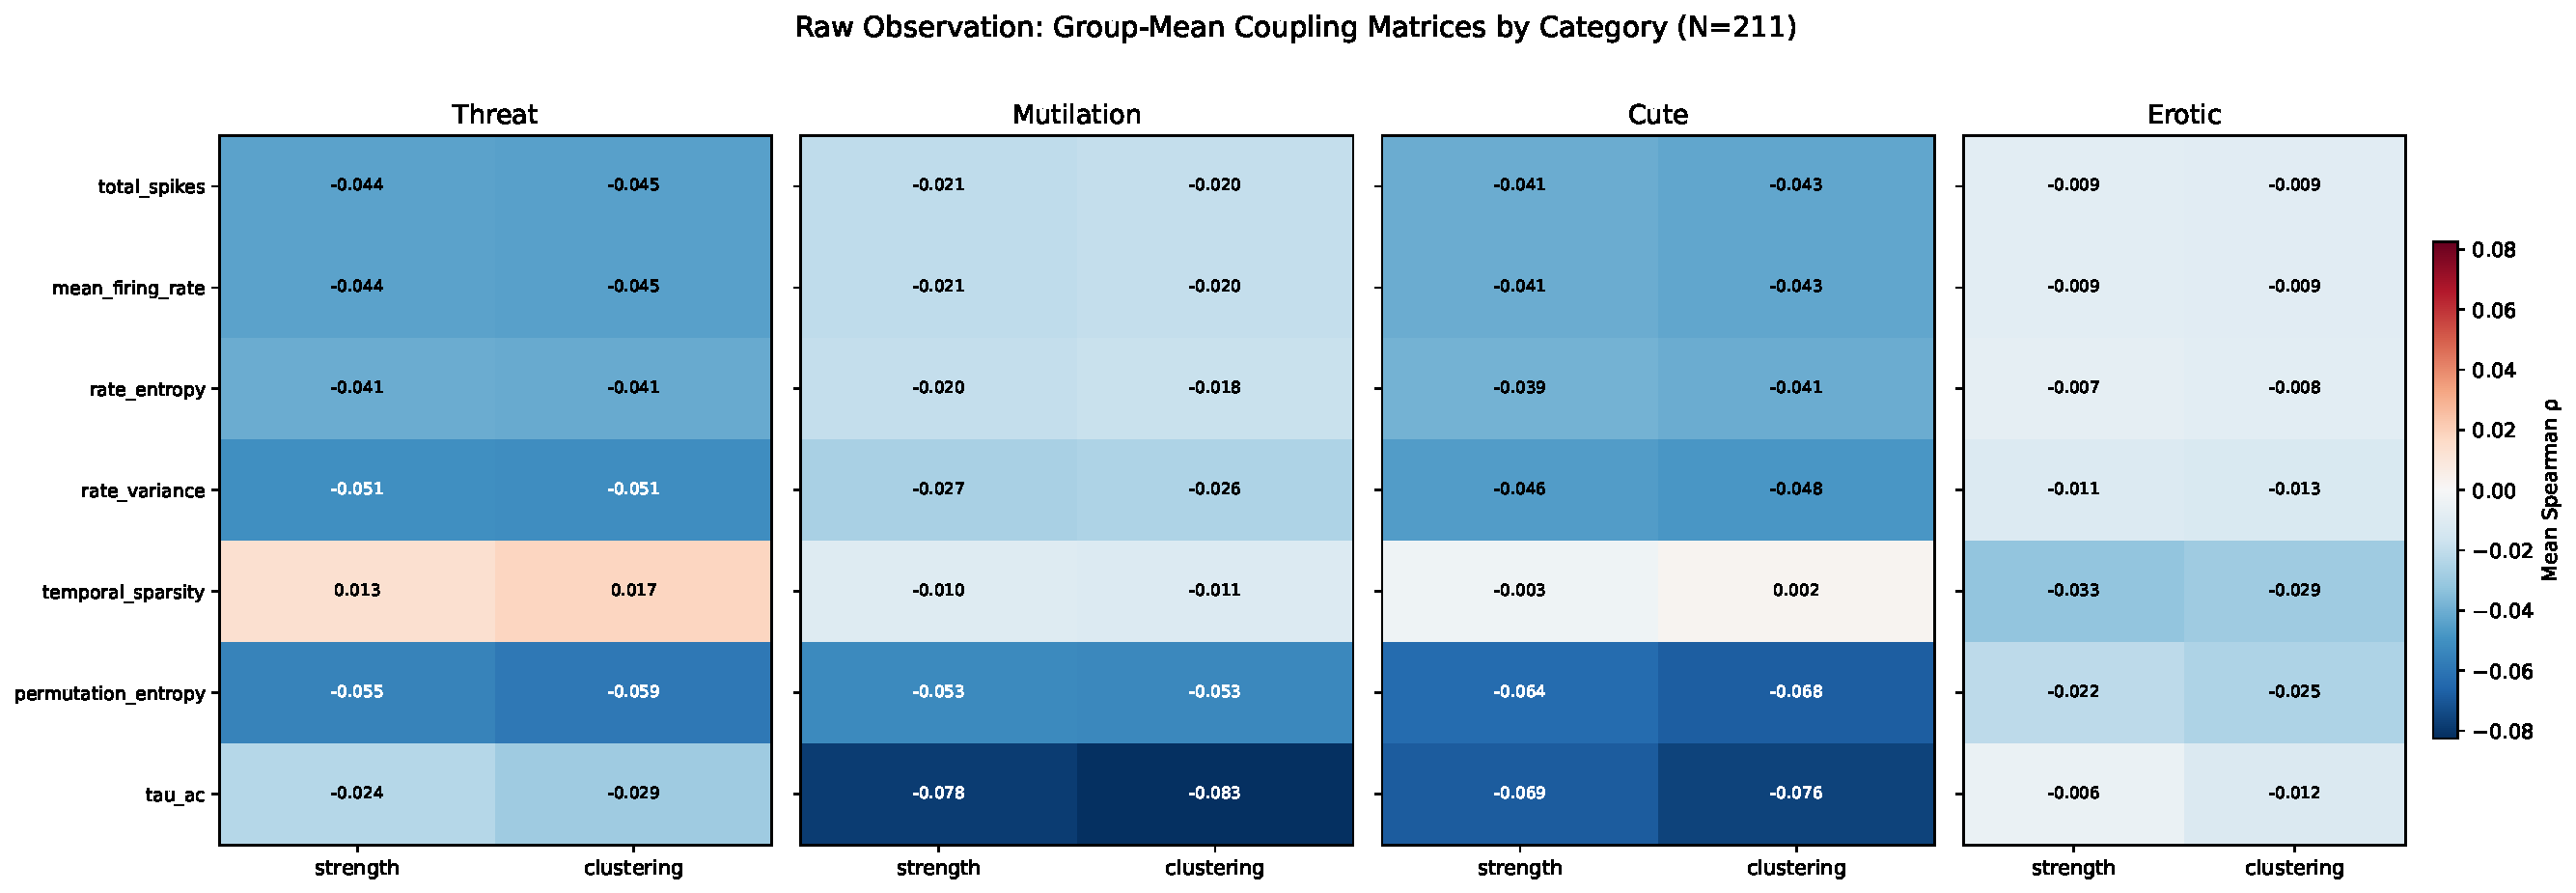
\includegraphics[width=0.95\textwidth]{pictures/chSynthesis/fig7_C1_category_C_matrices.pdf}
\caption{Group-mean coupling matrices by affective category ($N = 211$). Erotic shows the weakest coupling across all cells (most values near $-0.01$). Cute shows the strongest (permutation entropy $\times$ clustering $= -0.068$, $\tau_{AC} \times$ clustering $= -0.077$). Threat and Mutilation fall between, with different internal structures.}
\label{fig:category_C}
\end{figure}

Figure~\ref{fig:category_C} reveals a gradient across the four categories. The Erotic coupling matrix is the flattest: most entries near $-0.01$. Cute produces the strongest coupling, with permutation entropy $\times$ clustering at $-0.068$ and $\tau_{AC} \times$ clustering at $-0.077$. Threat and Mutilation fall between them but differ in internal structure: Threat has stronger amplitude-metric coupling, while Mutilation has stronger $\tau_{AC}$ coupling ($-0.083$).

\begin{figure}[htbp]
\centering
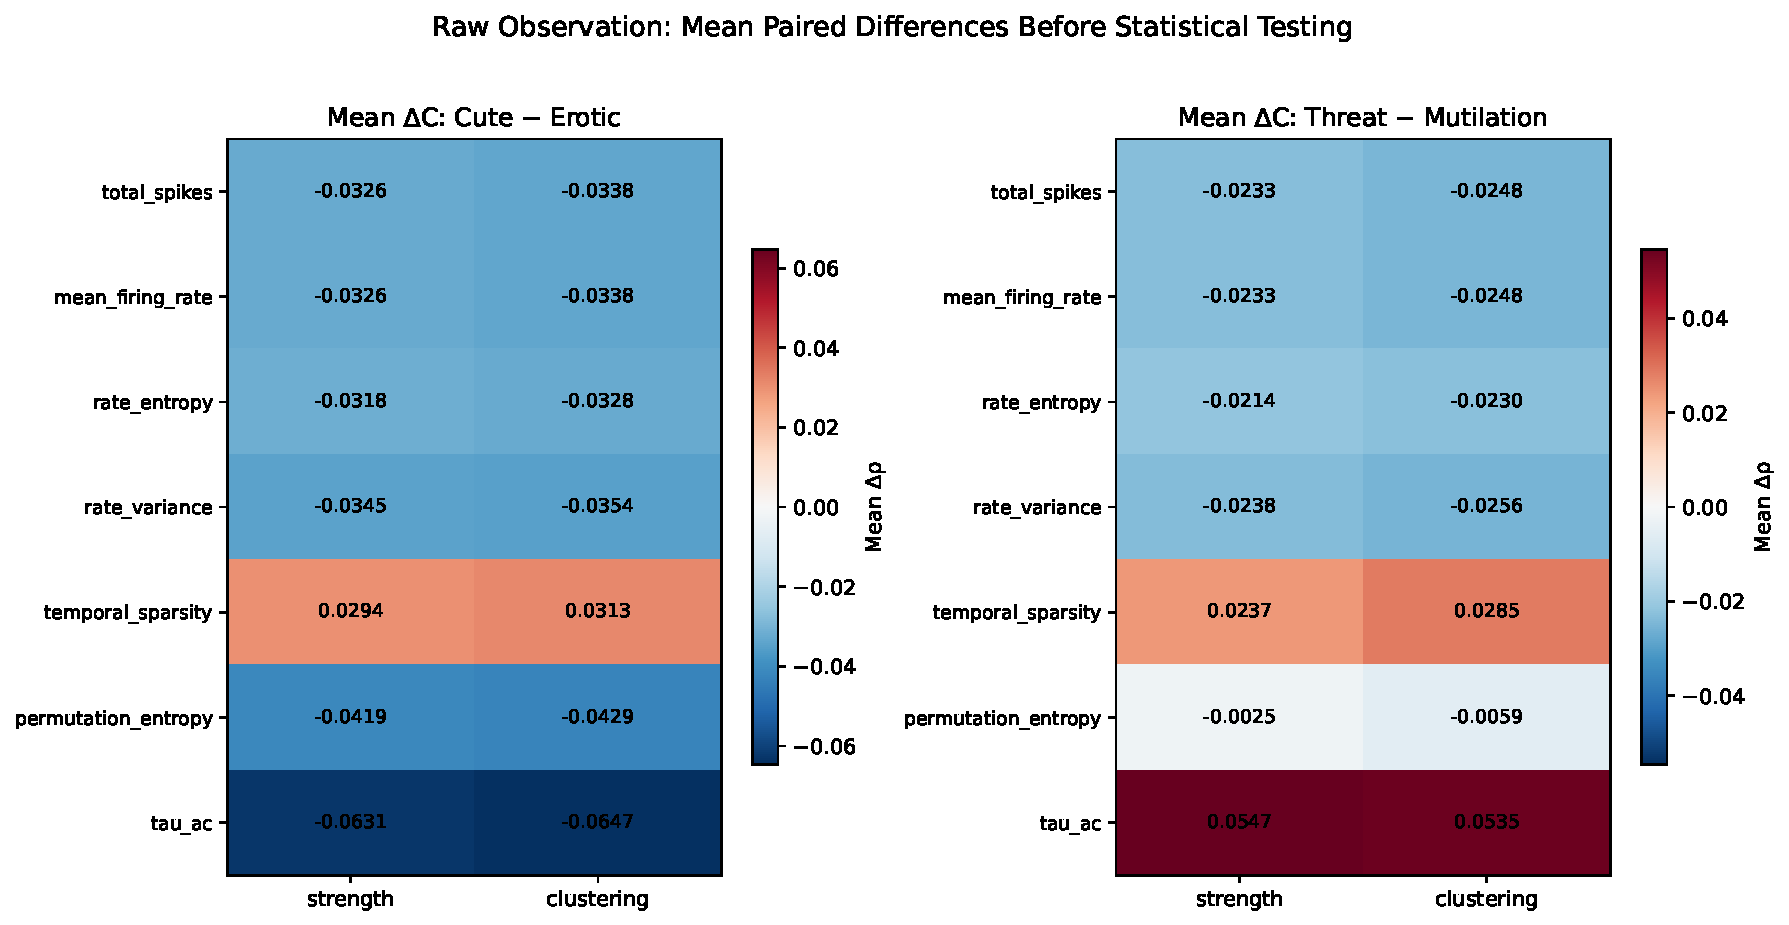
\includegraphics[width=0.95\textwidth]{pictures/chSynthesis/fig7_C2_raw_difference_matrices.pdf}
\caption{Mean paired difference matrices before statistical testing. Left: Cute $-$ Erotic shows consistent negative shifts (12 of 14 cells negative), with the largest differences in $\tau_{AC} \times$ clustering ($\Delta\rho = -0.065$) and $\tau_{AC} \times$ strength ($\Delta\rho = -0.063$). Right: Threat $-$ Mutilation shows a mixed pattern with $\tau_{AC}$ shifting in the opposite direction ($\Delta\rho = +0.054$).}
\label{fig:raw_diff_C}
\end{figure}

The raw Cute--Erotic paired differences (Figure~\ref{fig:raw_diff_C}) are negative in 12 of 14 cells, with only 43.1--46.9\% of subjects showing positive $\Delta\rho$ on the largest cells. The $\tau_{AC}$ row carries the largest shifts: $\Delta\rho = -0.065$ for $\tau_{AC} \times$ clustering and $-0.063$ for $\tau_{AC} \times$ strength.

\subsection{Quantitative Analysis}

\begin{figure}[htbp]
\centering
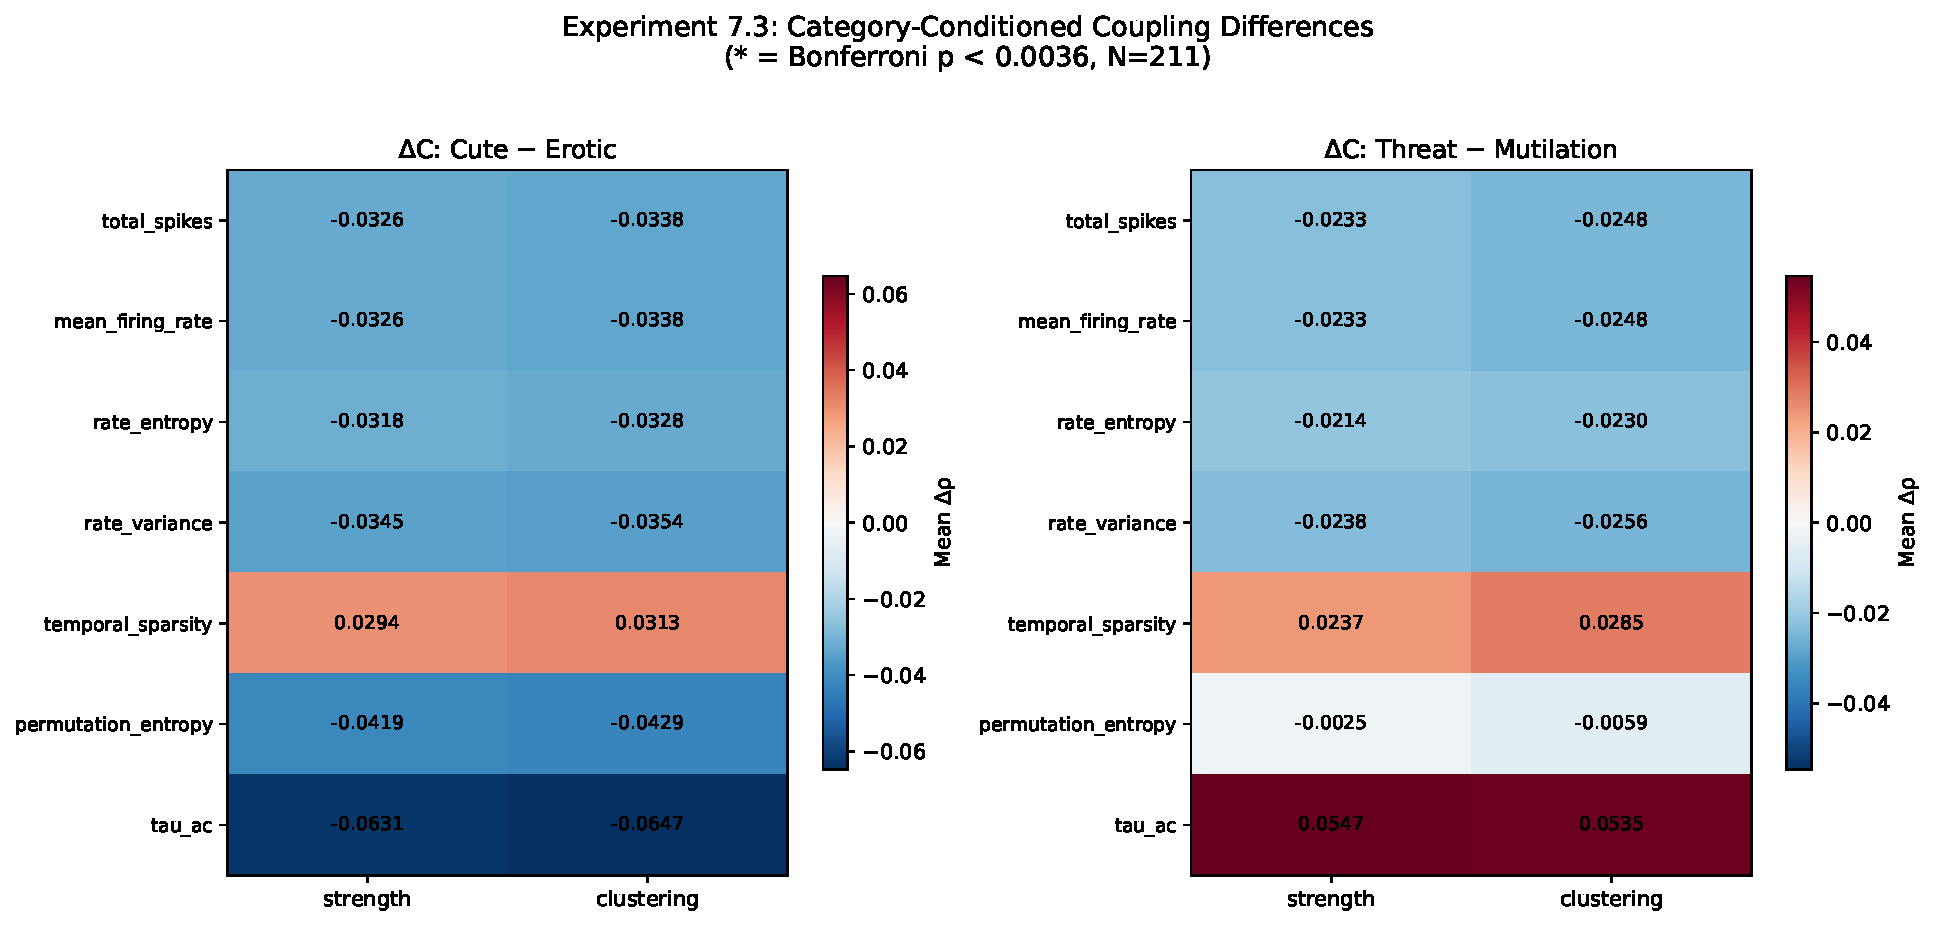
\includegraphics[width=0.95\textwidth]{pictures/chSynthesis/fig7_C3_difference_significance.pdf}
\caption{Difference matrices with Bonferroni significance masking ($\alpha = 0.05/14$). No individual cell reaches Bonferroni significance for either contrast. The $\tau_{AC}$ cells for Cute $-$ Erotic reach $p = 0.013$--$0.016$ uncorrected.}
\label{fig:diff_significance}
\end{figure}

No individual cell reaches Bonferroni significance for either within-valence contrast (0 of 14 for both; Figure~\ref{fig:diff_significance}). The closest are $\tau_{AC} \times$ clustering ($p = 0.013$, $d_z = 0.161$) and $\tau_{AC} \times$ strength ($p = 0.016$, $d_z = 0.155$) for Cute $-$ Erotic. The pattern-level Frobenius test is also non-significant (Cute $-$ Erotic: $\|\Delta\mathbf{C}\|_F = 0.150$, $p = 0.177$; Threat $-$ Mutilation: $\|\Delta\mathbf{C}\|_F = 0.109$, $p = 0.277$).

The metric-family decomposition reveals a gradient: temporal-structure metrics ($\hat{H}_\pi$, $\tau_{AC}$) carry the largest Cute--Erotic shifts (mean $|d_z| = 0.129$, min $p = 0.013$), approximately $1.8\times$ the amplitude-tracking family (mean $|d_z| = 0.072$, min $p = 0.237$).

\subsection{Interpretation and Significance}

The scalar $\kappa$ difference from Experiment~7.2 (Cute--Erotic $p = 0.025$) is distributed across the full $\mathbf{C}$ matrix as coordinated low-amplitude shifts in 12 of 14 cells rather than concentrated in one or two relationships. Each cell contributes a small consistent shift that sums to a detectable scalar difference but is individually underpowered after Bonferroni correction. Affective modulation of coupling operates at the pattern level rather than the individual-relationship level.

The temporal-structure metrics---the same metrics that Chapter~\ref{chap:dynamics} Experiment~6.4 identified as maximally sensitive to genuine phase-dependent temporal organization---are the ones whose topological alignment shifts most under different affective conditions. This cross-chapter convergence is specific: the LIF reservoir's distinctive measurement contribution (temporal-structure sensitivity) is the channel through which affective modulation of coupling operates.

For the Threat--Mutilation contrast, $\tau_{AC}$ shows the opposite pattern: Threat produces \emph{weaker} $\tau_{AC}$ coupling than Mutilation ($\Delta\rho = +0.054$, $p = 0.024$ uncorrected). The autocorrelation decay metric's topological alignment shifts in opposite directions for the two valence pairs, indicating that coupling reorganization is content-specific rather than reflecting a generic arousal scaling.

The $\tau_{AC}$ cells at $d_z \approx 0.16$ would require approximately $N = 480$ to reach Bonferroni significance, providing a concrete target for future replication. A natural question follows: although the omnibus category effect is not significant, does the 29.2\% between-subject variance in $\kappa$ contain diagnosis-associated structure?


\section{Experiment 7.4: Diagnosis-Associated Coupling Differences}
\label{sec:exp7_diagnosis}

\subsection{Mathematical Motivation}

Chapter~\ref{chap:dynamics} Experiment~6.6 identified three distinguishable diagnosis-associated temporal descriptor patterns: SUD category-dependent reduction, ADHD category-independent elevation, and MDD positive-selective elevation. Chapter~5 identified SUD as the strongest graph-topological phenotype. The question is whether these diagnosis-associated differences in the temporal domain and the spatial domain also manifest as differences in their alignment. The observable quantity is $\Delta\bar{\kappa} = \bar{\kappa}_{\text{Dx}^+} - \bar{\kappa}_{\text{Dx}^-}$ for each of five diagnoses, where $\bar{\kappa}_s = \frac{1}{4}\sum_c \kappa_{s,c}$ is the subject-averaged coupling strength.

All diagnosis comparisons are one-versus-rest within a transdiagnostic sample with mean comorbidity of 2.0 diagnoses per subject. Results are diagnosis-associated coupling differences conditioned by the comorbidity structure, not disorder-specific signatures.

\subsection{Experimental Design}

Five diagnoses are tested: MDD ($n^+ = 142$, $n^- = 64$), SUD ($n^+ = 85$, $n^- = 121$), PTSD ($n^+ = 82$, $n^- = 124$), GAD ($n^+ = 60$, $n^- = 146$), and ADHD ($n^+ = 50$, $n^- = 156$). Group comparisons use Mann--Whitney~$U$ on $\bar{\kappa}_s$ with Bonferroni correction across five tests ($\alpha = 0.01$). A secondary analysis tests diagnosis $\times$ category interactions by permutation (2,000 iterations). Power analysis reports the minimum detectable Cohen's~$d$ at $\alpha = 0.05$, power $= 0.80$ for each comparison.

\subsection{Raw Observation}

\begin{figure}[htbp]
\centering
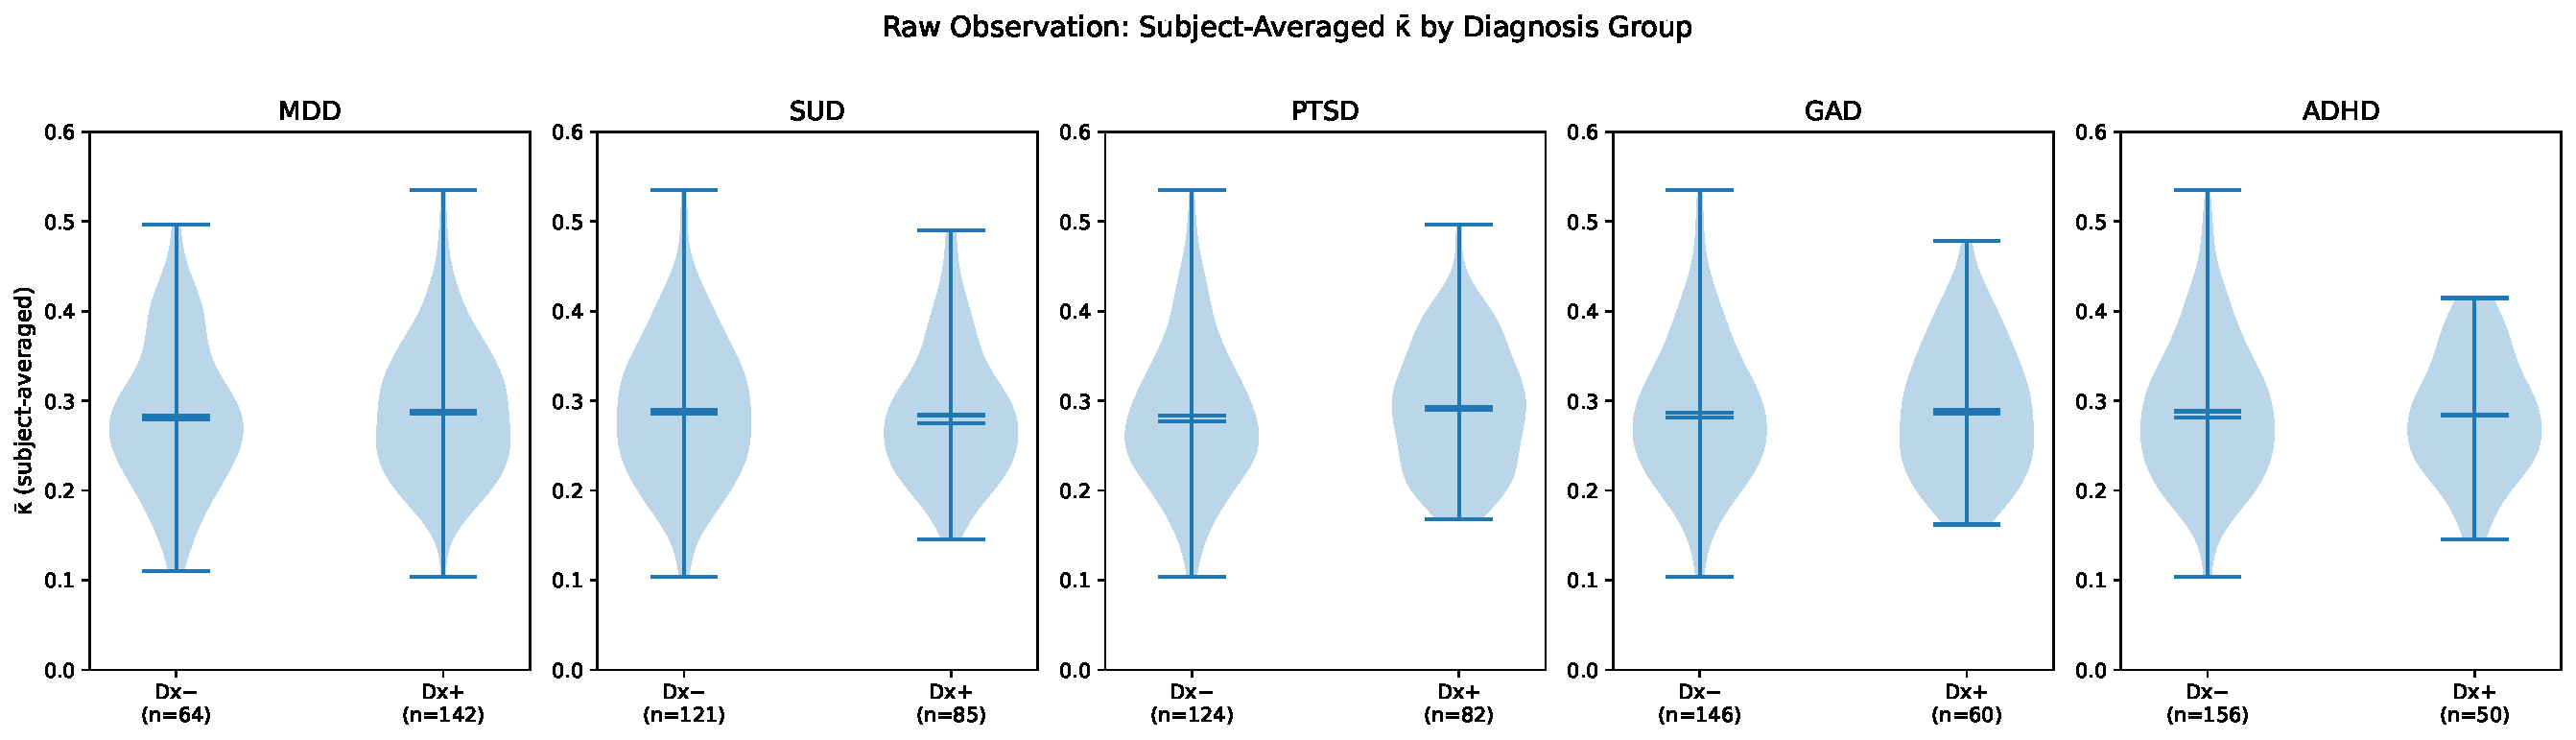
\includegraphics[width=0.95\textwidth]{pictures/chSynthesis/fig7_D1_raw_diagnosis_kappa.pdf}
\caption{Subject-averaged $\bar{\kappa}$ by diagnosis group for five diagnoses. The Dx$^+$ and Dx$^-$ distributions overlap extensively for all diagnoses. No visible separation is present in the raw violin plots.}
\label{fig:raw_diag_kappa}
\end{figure}

The raw violin plots (Figure~\ref{fig:raw_diag_kappa}) show near-complete distributional overlap between Dx$^+$ and Dx$^-$ for all five diagnoses. Group means differ by at most 0.009 (PTSD: $\bar{\kappa}_{\text{Dx}^+} = 0.293$ versus $\bar{\kappa}_{\text{Dx}^-} = 0.284$). The within-group standard deviations ($\approx 0.07$) are an order of magnitude larger than the between-group mean differences.

\subsection{Quantitative Analysis}

\begin{table}[htbp]
\centering
\caption{Diagnosis-associated coupling differences (Experiment~7.4).}
\label{tab:diagnosis_coupling}
\small
\begin{tabular}{lccccccc}
\toprule
\textbf{Dx} & \textbf{$n^+$} & \textbf{$n^-$} & \textbf{$\bar{\kappa}^+$} & \textbf{$\bar{\kappa}^-$} & \textbf{$d$} & \textbf{$p$} & \textbf{MDE} \\
\midrule
MDD  & 142 & 64  & 0.289 & 0.283 & $+0.081$ & 0.609 & 0.42 \\
SUD  & 85  & 121 & 0.284 & 0.290 & $-0.075$ & 0.485 & 0.40 \\
PTSD & 82  & 124 & 0.293 & 0.284 & $+0.116$ & 0.322 & 0.40 \\
GAD  & 60  & 146 & 0.290 & 0.287 & $+0.043$ & 0.762 & 0.43 \\
ADHD & 50  & 156 & 0.285 & 0.288 & $-0.051$ & 0.921 & 0.46 \\
\bottomrule
\end{tabular}
\end{table}

No diagnosis reaches significance (Table~\ref{tab:diagnosis_coupling}). All Cohen's~$d$ values are below 0.12, well below the minimum detectable effect (MDE) of $d \approx 0.40$--$0.46$ for these sample sizes. The effects are not marginal---they are absent at the scalar $\bar{\kappa}$ level.

\begin{figure}[htbp]
\centering
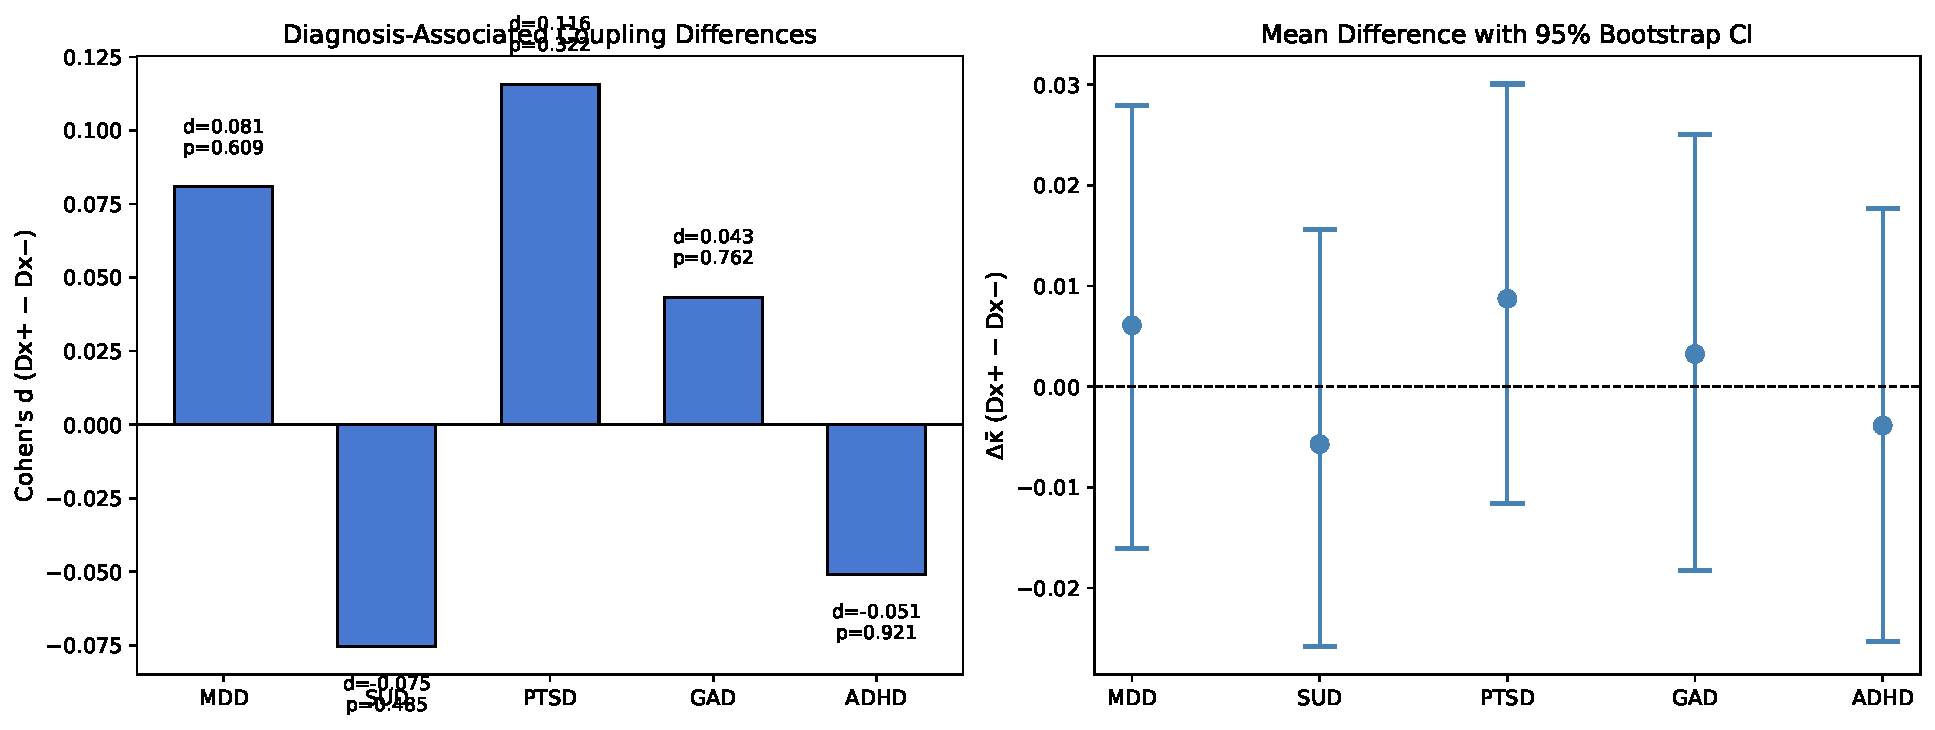
\includegraphics[width=0.95\textwidth]{pictures/chSynthesis/fig7_D2_diagnosis_effects.pdf}
\caption{Left: Cohen's~$d$ for each diagnosis. All values are below $|d| = 0.12$. Right: bootstrap 95\% confidence intervals for the mean $\bar{\kappa}$ difference. All intervals include zero.}
\label{fig:diagnosis_effects}
\end{figure}

The secondary diagnosis $\times$ category interaction analysis identifies one suggestive pattern: ADHD shows a category-dependent coupling profile with the lowest $\kappa$ for Mutilation (0.261) and the highest for Erotic (0.308), reaching $p = 0.035$ uncorrected. This does not survive Bonferroni correction across five diagnoses and is carried forward as a hypothesis for future investigation.

\subsection{Interpretation and Significance}

The between-subject variance in $\kappa$ (29.2\% from Experiment~7.2) is not organized along diagnosis boundaries for any of the five tested conditions. This is an informative observation: Chapters~5 and~\ref{chap:dynamics} both found diagnosis-associated effects at the individual descriptor level (graph topology and dynamical metrics separately). The coupling statistic, which measures their \emph{alignment}, does not carry the same diagnosis-associated signal. Clinical populations may differ in their temporal descriptors (Chapter~\ref{chap:dynamics}) and their topological descriptors (Chapter~5) while maintaining similar temporal--spatial alignment. The coupling layer accesses a different dimension of signal organization than either individual layer.

The ADHD interaction ($p = 0.035$ uncorrected) converges with Chapter~\ref{chap:dynamics}'s finding that ADHD produces category-independent dynamical elevation: if the temporal descriptors are uniformly elevated while the topological descriptors are category-dependent, the coupling profile may shift in a category-specific way. This remains a hypothesis.

A natural question follows: if coupling is organizationally informative but not diagnosis-discriminative at the scalar level, do the individual descriptor families carry complementary discriminative information when combined?


\section{Experiment 7.5: Augmentation Ablation}
\label{sec:exp7_augmentation}

\subsection{Mathematical Motivation}

Experiments~7.1--7.4 established that coupling exists, is observation-specific, and is not diagnosis-discriminative at the $\bar{\kappa}$ level. Chapter~\ref{chap:dynamics} established that dynamical descriptors are ``analytically informative rather than discriminatively additive at the linear-readout level.'' The question for this experiment is whether combining topological and dynamical descriptor families in a single flat feature vector improves clinical detection beyond either family alone. If the combination improves performance, the two families carry complementary discriminative information that a linear readout can exploit. If not, their value is organizational---the coupling structure characterized in Experiments~7.1--7.3---rather than discriminatively additive.

\subsection{Experimental Design}

Four feature conditions are constructed from subject-averaged per-electrode descriptors: T-only (68 features: 34 electrodes $\times$ 2 topology metrics), D-only (238 features: 34 electrodes $\times$ 7 dynamical metrics), T+D (306 features: concatenation), and T+D+$\kappa$ (307 features: concatenation plus subject-averaged coupling strength). Five binary detection tasks are tested: SUD, MDD, PTSD, GAD, and ADHD. The primary readout is $L_2$-regularized logistic regression ($C = 1.0$) with subject-level stratified 5-fold cross-validation repeated 10 times (50 total folds).

\subsection{Raw Observation}

\begin{figure}[htbp]
\centering
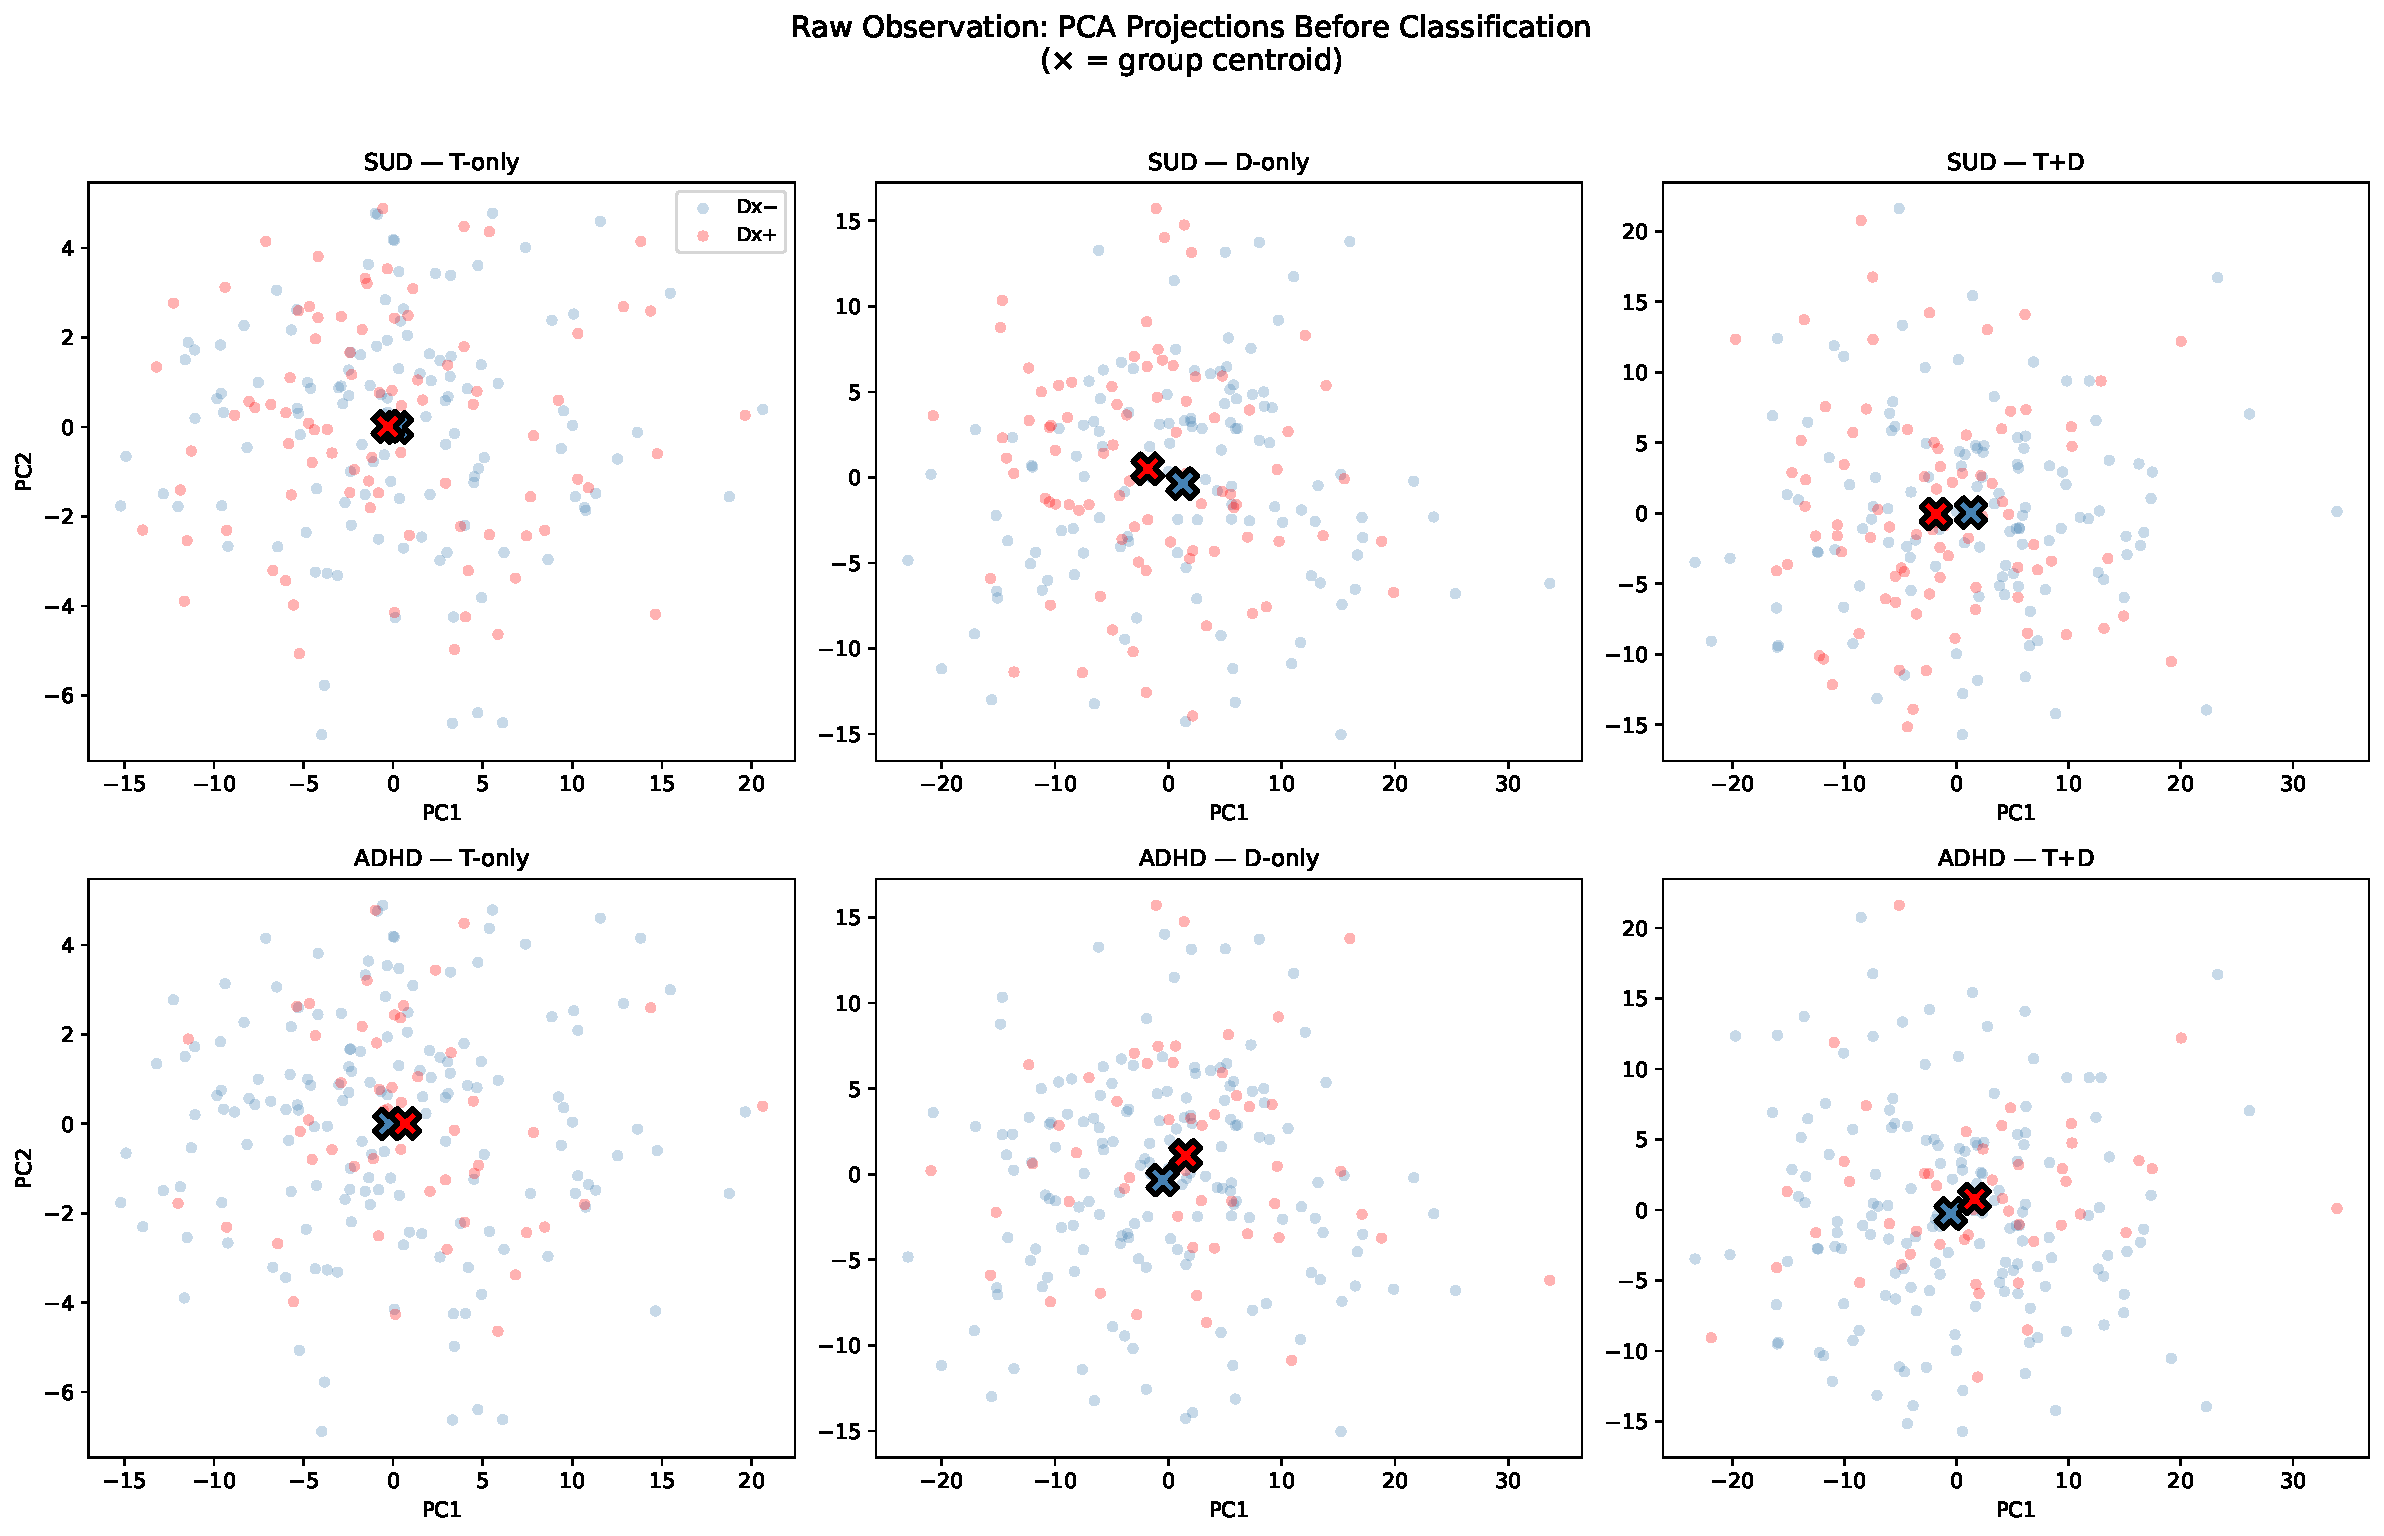
\includegraphics[width=0.95\textwidth]{pictures/chSynthesis/fig7_E1_raw_pca_projections.pdf}
\caption{PCA projections before classification for SUD (top) and ADHD (bottom) across T-only, D-only, and T+D feature spaces. Group centroids ($\times$) are marked. SUD shows near-complete overlap in all three spaces. ADHD shows visible D-only centroid offset that is absent in T-only.}
\label{fig:pca_projections}
\end{figure}

Three properties of the raw feature spaces are observable before any classifier is trained. First, the D-only feature matrix (238 features, $N = 211$) is rank-deficient: rank 211 of 238 columns. The T+D matrix (306 features) is even more constrained ($N/p = 0.69$). T-only ($N/p = 3.1$) is the only well-conditioned space. Second, PCA projections (Figure~\ref{fig:pca_projections}) show near-complete overlap between Dx$^+$ and Dx$^-$ for SUD across all three spaces, while ADHD shows a visible D-only centroid offset absent in T-only. Third, univariate screening reveals that zero of 68 topology features reach $p < 0.05$ for either SUD or ADHD, while 44 of 238 dynamics features reach $p < 0.05$ for SUD (concentrated at electrodes~28 and~3) and 29 of 238 for ADHD (concentrated at electrodes~14 and~33).

\begin{figure}[htbp]
\centering
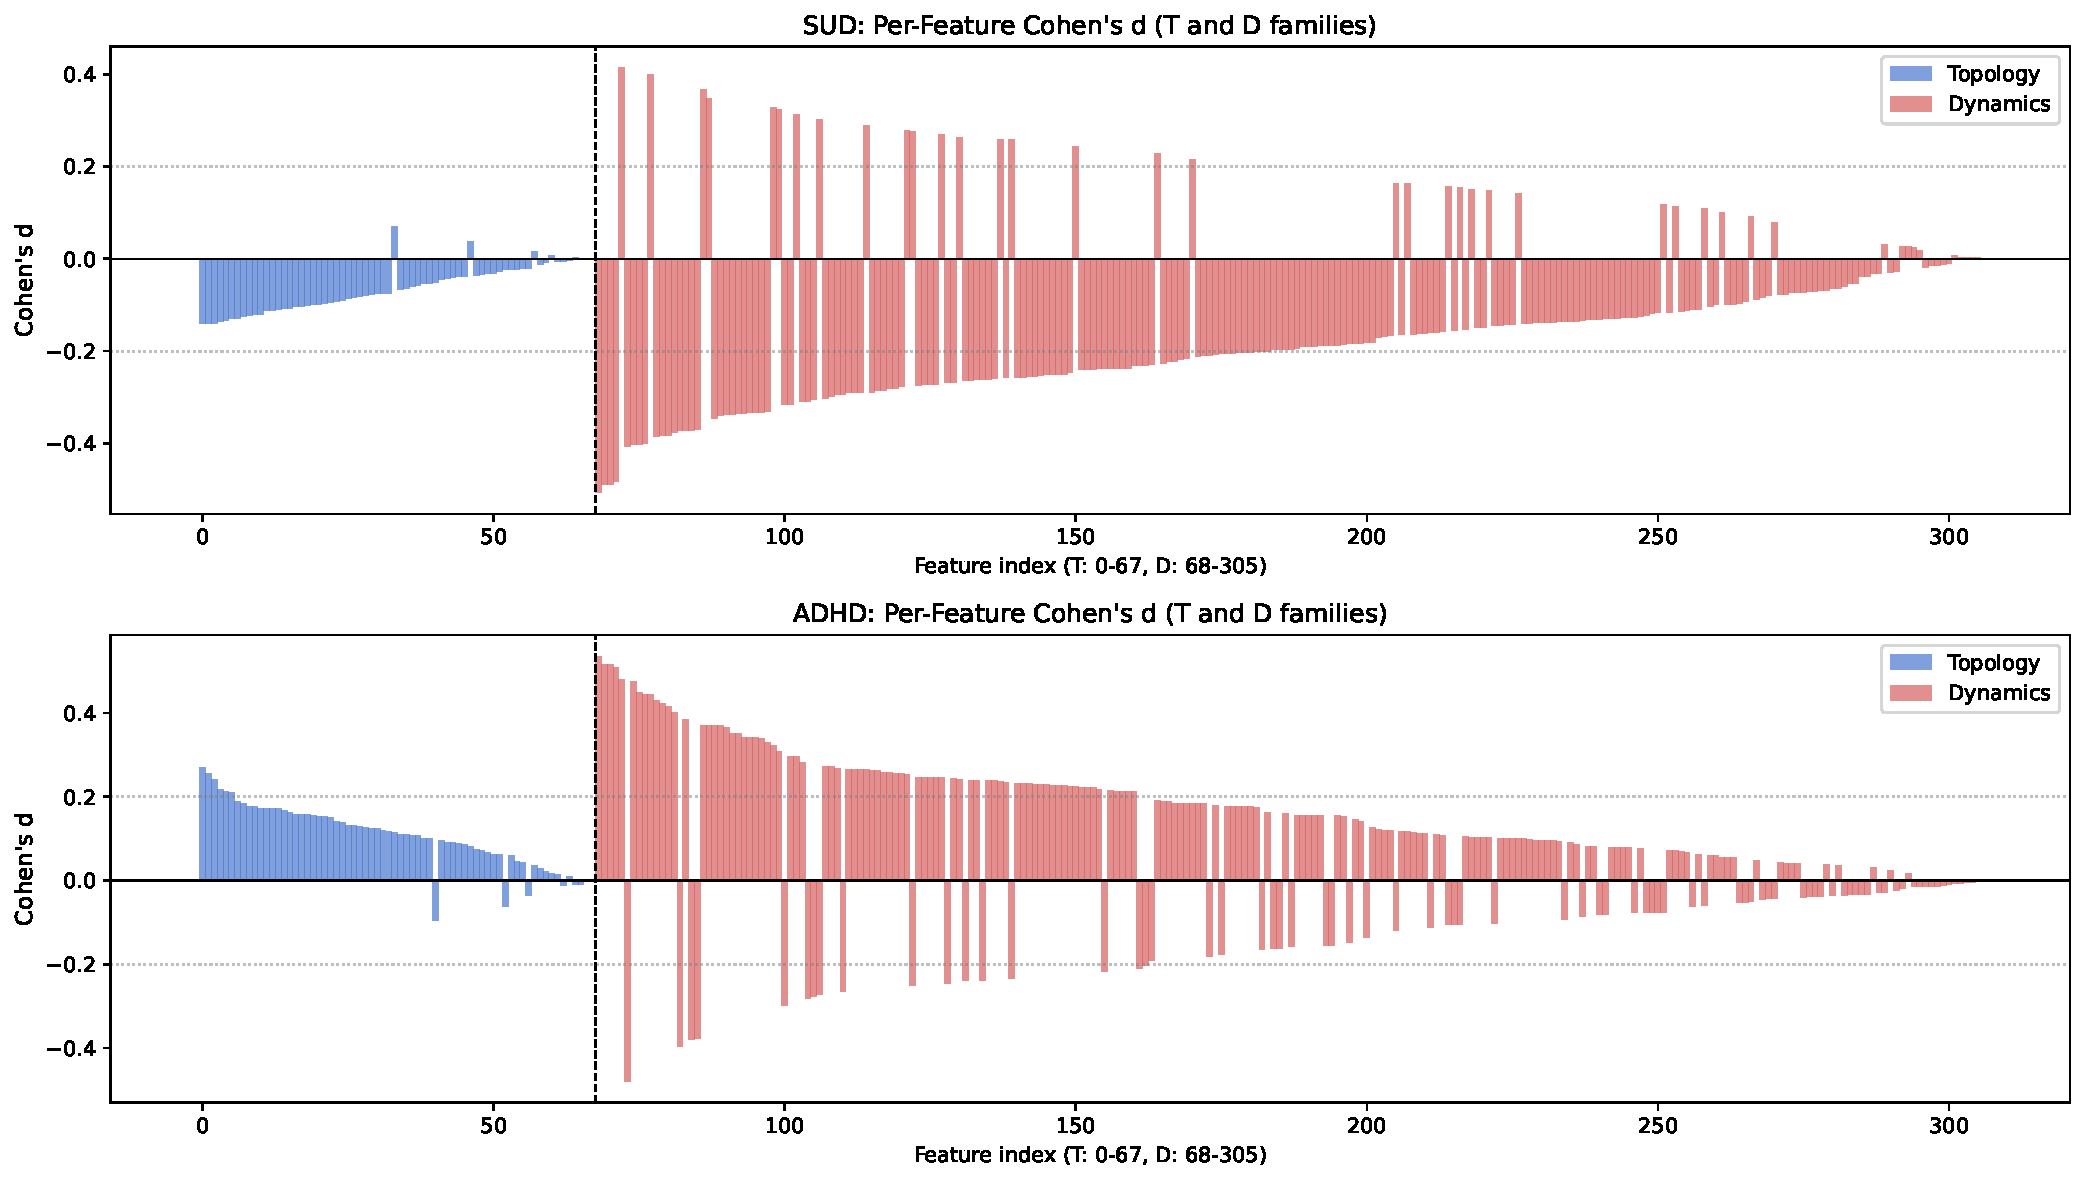
\includegraphics[width=0.95\textwidth]{pictures/chSynthesis/fig7_E2_raw_univariate_effects.pdf}
\caption{Per-feature Cohen's~$d$ across all 306 features for SUD (top) and ADHD (bottom). Topology features (left of vertical line) cluster near $d = 0$. Dynamics features (right) show scattered effects, broader for ADHD than SUD.}
\label{fig:univariate_effects}
\end{figure}

These raw observations predict three classification outcomes: SUD detection will be near chance (no visible separation); ADHD detection may succeed in D-only space (visible centroid offset, broader univariate effects); and concatenating uninformative topology features with dynamics will dilute signal in the rank-deficient combined space.

\subsection{Quantitative Analysis}

\begin{table}[htbp]
\centering
\caption{Augmentation ablation results: AUC $\pm$ SD across 50 CV folds (Experiment~7.5).}
\label{tab:augmentation}
\small
\begin{tabular}{lcccc}
\toprule
\textbf{Dx} & \textbf{T-only} & \textbf{D-only} & \textbf{T+D} & \textbf{T+D+$\kappa$} \\
\midrule
SUD  & $0.464 \pm 0.071$ & $0.464 \pm 0.076$ & $0.458 \pm 0.083$ & $0.455 \pm 0.082$ \\
MDD  & $0.518 \pm 0.094$ & $0.504 \pm 0.085$ & $0.512 \pm 0.092$ & $0.510 \pm 0.090$ \\
PTSD & $0.487 \pm 0.072$ & $0.527 \pm 0.073$ & $0.510 \pm 0.069$ & $0.505 \pm 0.069$ \\
GAD  & $\mathbf{0.581} \pm 0.092$ & $0.533 \pm 0.093$ & $0.568 \pm 0.084$ & $0.563 \pm 0.083$ \\
ADHD & $0.533 \pm 0.077$ & $\mathbf{0.622} \pm 0.086$ & $0.597 \pm 0.076$ & $0.608 \pm 0.084$ \\
\bottomrule
\end{tabular}
\end{table}

The classification results (Table~\ref{tab:augmentation}) confirm each prediction from the raw observation. SUD detection is at chance across all conditions (AUC $\approx 0.46$). ADHD D-only achieves AUC $= 0.622$---the highest value in the experiment---while T-only achieves only $0.533$. GAD shows the inverse: T-only achieves $0.581$, D-only $0.533$. For every diagnosis, T+D is equal to or lower than the better individual family; concatenation never improves classification.

\begin{figure}[htbp]
\centering
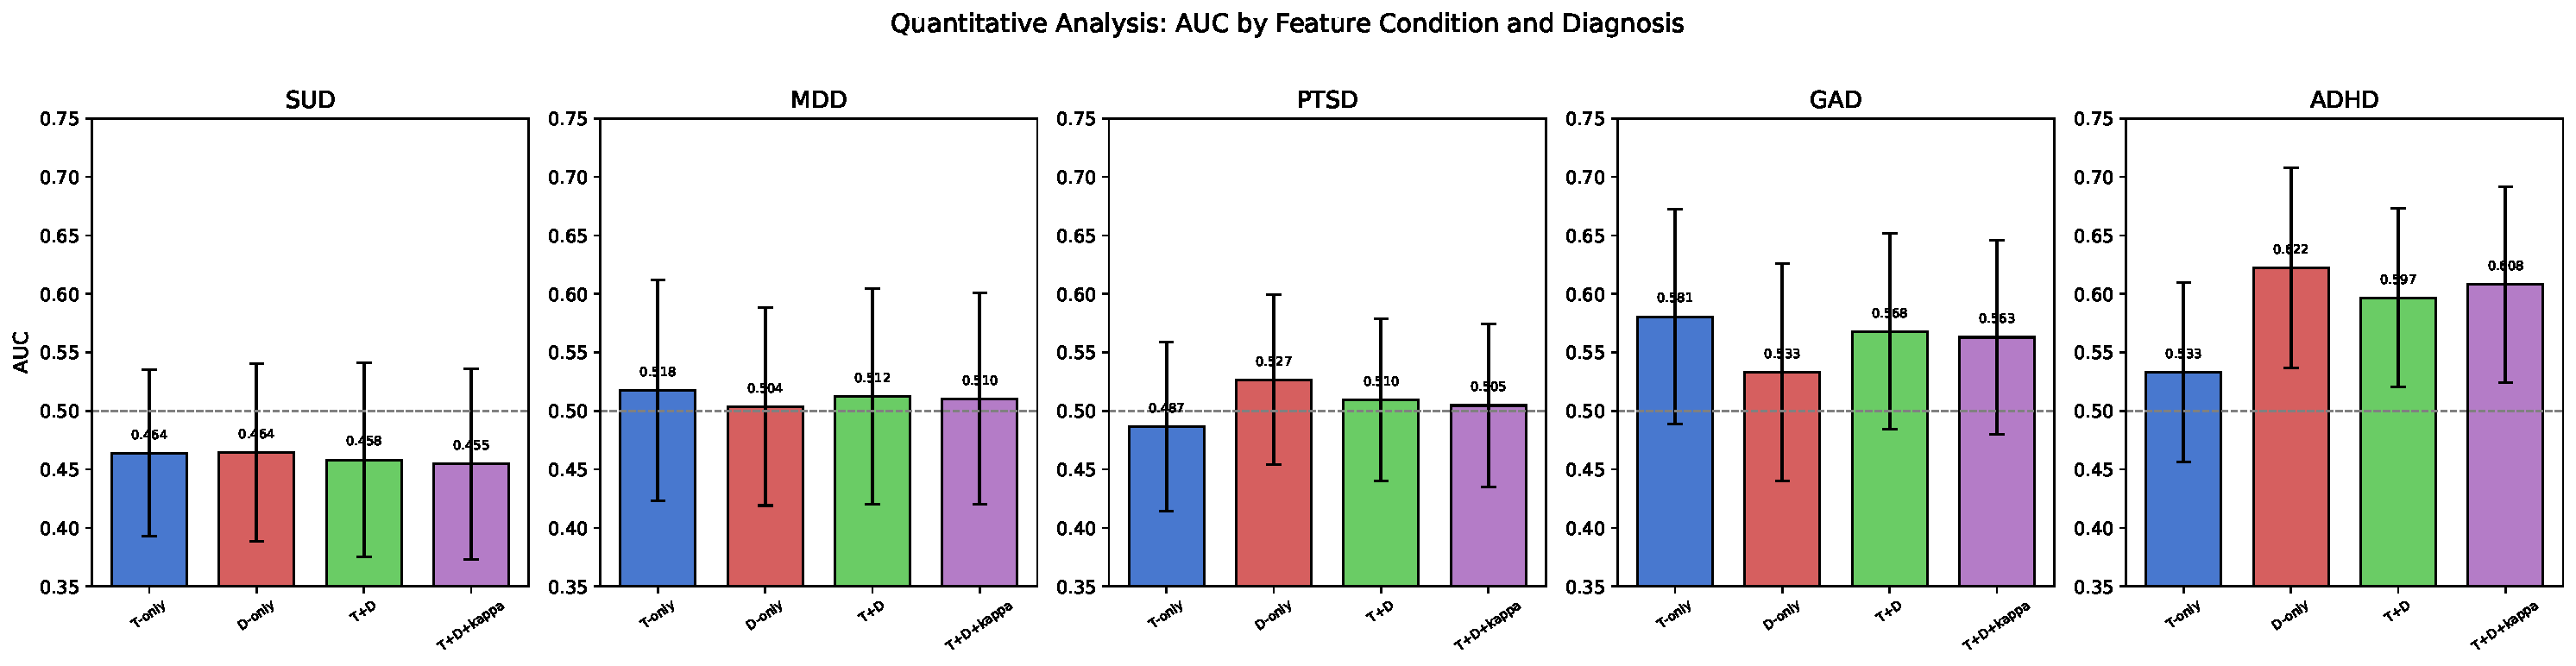
\includegraphics[width=0.95\textwidth]{pictures/chSynthesis/fig7_E4_classification_auc.pdf}
\caption{AUC by feature condition and diagnosis. Bold values indicate the best condition per diagnosis. ADHD D-only and GAD T-only are the two results meaningfully above chance.}
\label{fig:classification_auc}
\end{figure}

Adding uninformative topology features to the dynamics signal for ADHD degrades performance from $0.622$ to $0.597$ ($p = 5.1 \times 10^{-4}$). Adding the scalar $\kappa$ partially recovers it: T+D+$\kappa$ $= 0.608$ versus T+D $= 0.597$ ($p = 1.4 \times 10^{-3}$), indicating that coupling strength carries non-redundant ADHD information that neither individual descriptor family provides.

\subsection{Interpretation and Significance}

The central finding is that concatenation never improves over the better individual family for any diagnosis. The dynamical and topological descriptor families do not carry complementary discriminative information at the linear-readout level. Their value is organizational---the coupling structure revealed by Experiments~7.1--7.3---rather than discriminatively additive. This confirms the Chapter~\ref{chap:dynamics} observation that dynamical descriptors are analytically informative rather than classification-enhancing, and extends it to the combined temporal--spatial feature space.

The diagnosis-specificity of descriptor families is itself a finding: ADHD is best captured by dynamics ($0.622$), GAD by topology ($0.581$). Different clinical dimensions are accessed by different axes of the ARSPI-Net instrument. A complete clinical characterization requires both axes, not because they combine additively, but because they measure different properties of the underlying EEG.

The $\kappa$ augmentation effect for ADHD ($p = 0.001$) converges with Experiment~7.4's ADHD $\times$ category interaction ($p = 0.035$ uncorrected). Across two independent analyses, ADHD is the one diagnosis where the coupling layer carries information beyond what the individual descriptor families provide. This makes ADHD the strongest candidate for coupling-derived clinical characterization in future work.


\section{Three-Class Replication and Cross-Granularity Comparison}
\label{sec:ch7_3class}

The four-class experiments in Sections~\ref{sec:exp7_coupling}--\ref{sec:exp7_augmentation} provide within-valence resolution (Threat vs.\ Mutilation, Cute vs.\ Erotic) that reveals subcategory-specific coupling phenomena. This section replicates the five core analyses at three-class resolution (Negative, Neutral, Pleasant), where the $3.6\times$ stronger condition signal ($8.7\%$ vs.\ $2.4\%$ condition variance in the embedding space) provides tighter confidence intervals for all coupling measurements. All figures are presented inline; supplementary visualizations are in Appendix~\ref{app:ch7_figs}.

\subsection{Coupling Existence at Three-Class}

The mean coupling scalar at three-class is $\kappa = 0.221 \pm 0.111$, with the permutation test producing $p = 0.000$ ($0/1{,}000$ null realizations exceed the observed value). Coupling is unambiguously real at both granularities (Figure~\ref{fig:ch7_3class_coupling}).

The coupling matrix at three-class reveals a more nuanced pattern than the uniformly negative four-class result. Of the $14$ entries, $6$ are negative and $8$ are positive. Rate variance ($+0.100$ with strength), temporal sparsity ($+0.107$), and $\tau_{AC}$ ($+0.088$) are \emph{positively} coupled with connectivity---high-connectivity channels produce more variable, sparser, and more persistent reservoir dynamics. Total spikes ($-0.054$) and MFR ($-0.054$) are negatively coupled---high-connectivity channels fire fewer but more temporally structured spikes. The reservoir responds to phase-locked input with qualitatively different dynamics than to independent input.

\begin{figure}[H]
    \centering
    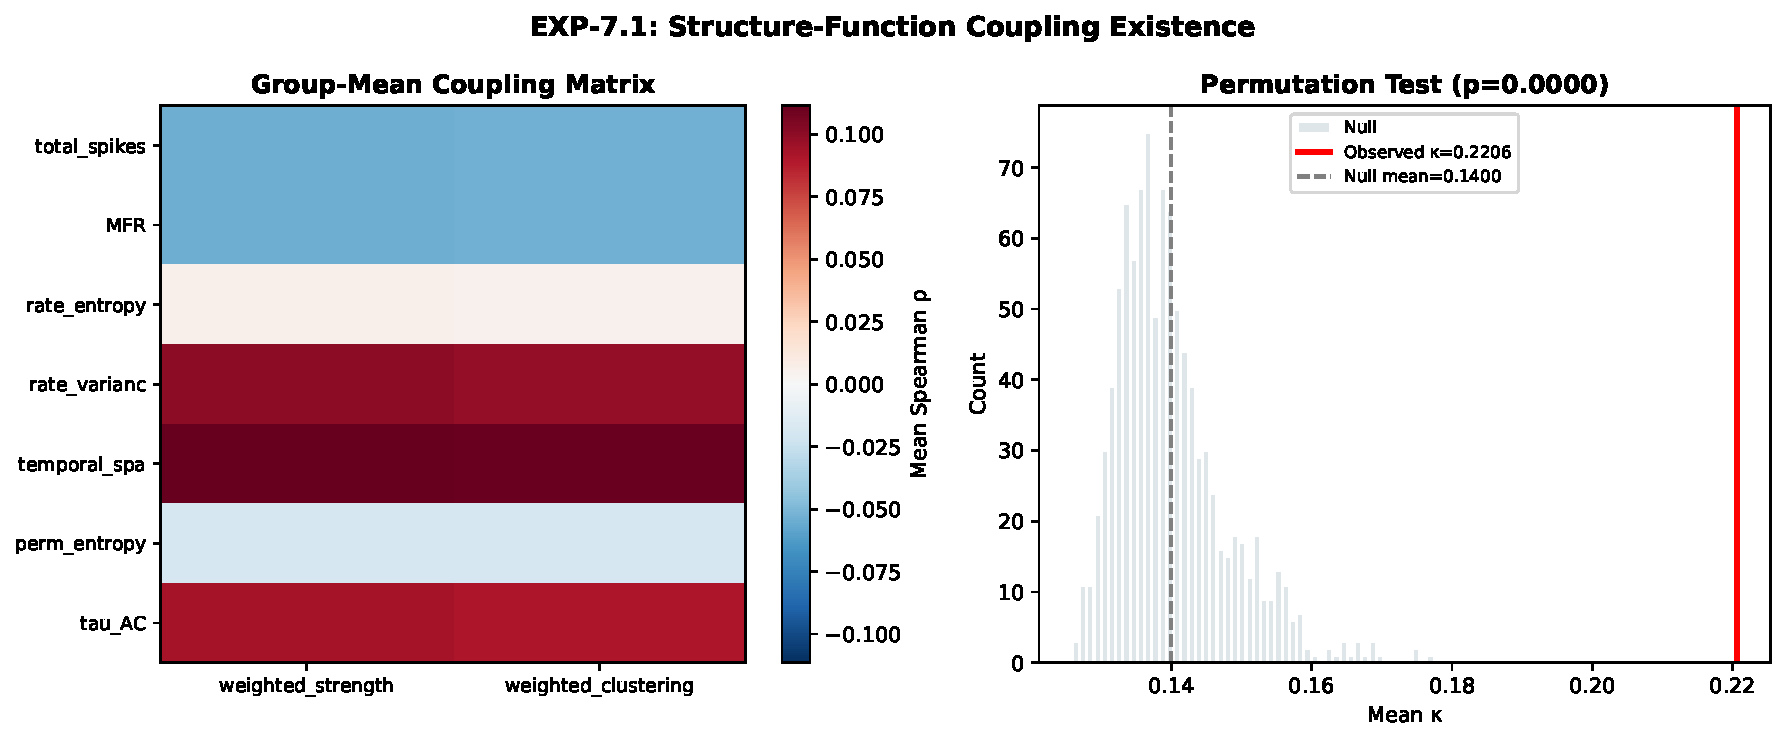
\includegraphics[width=\textwidth]{pictures/chSynthesis/fig_3class_coupling_existence.pdf}
    \caption{Coupling existence at three-class resolution ($N = 211$, $633$ observations). Left: group-mean $7 \times 2$ coupling matrix showing mixed positive/negative pattern ($6/14$ negative, $8/14$ positive), contrasting with the uniformly negative four-class result. Right: permutation test ($1{,}000$ shuffles). Observed $\kappa = 0.221$ exceeds every null realization ($p = 0.000$).}
    \label{fig:ch7_3class_coupling}
\end{figure}

\subsection{Variance Decomposition at Three-Class}

Subject accounts for $40.3\%$ of $\kappa$ variance, condition for $0.7\%$, and residual for $59.0\%$ (Figure~\ref{fig:ch7_3class_variance}). The condition effect does not reach significance ($F = 2.33$, $p = 0.101$) but trends closer than the four-class result ($p = 0.133$). The subject fraction ($40.3\%$) is higher than the four-class value ($29.2\%$), while the residual fraction ($59.0\%$) is lower than the four-class value ($70.1\%$). The stronger condition signal at three-class concentrates more variance in the subject component and less in the observation-specific residual.

\begin{figure}[H]
    \centering
    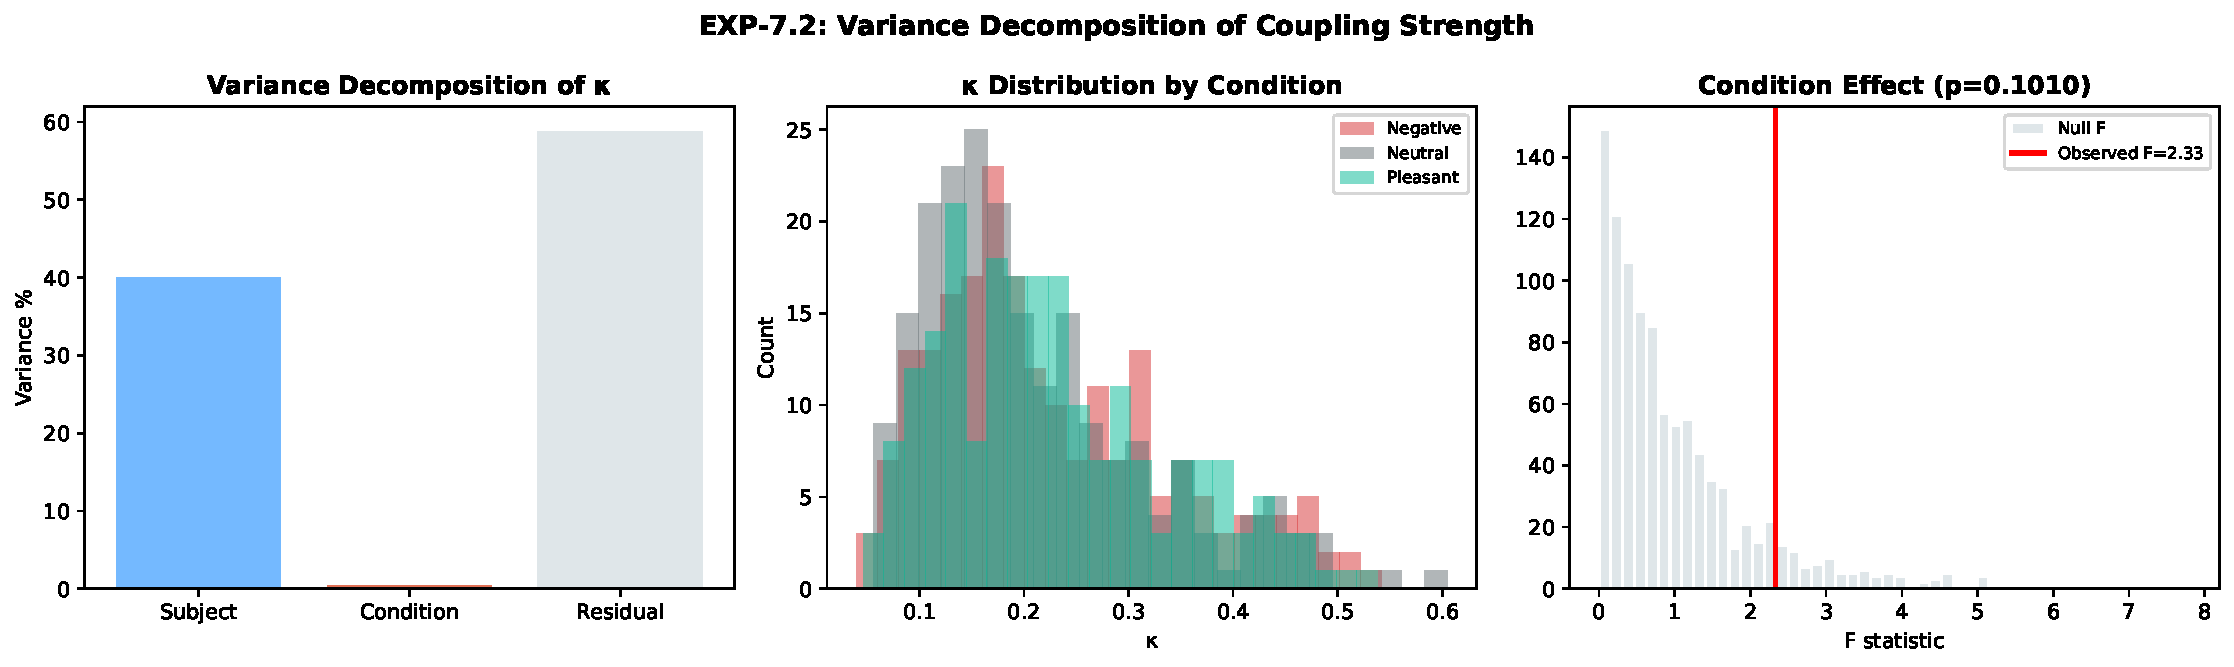
\includegraphics[width=\textwidth]{pictures/chSynthesis/fig_3class_variance_decomposition.pdf}
    \caption{Variance decomposition of coupling strength $\kappa$ at three-class. Left: subject $40.3\%$, condition $0.7\%$, residual $59.0\%$. Center: $\kappa$ distributions by condition. Right: condition $F$-test permutation null ($p = 0.101$). The condition fraction trends larger than at four-class ($0.6\%$, $p = 0.133$) but does not reach significance.}
    \label{fig:ch7_3class_variance}
\end{figure}

\subsection{Clinical Coupling at Three-Class}

No diagnosis produces a significant difference in $\kappa$ at three-class (Figure~\ref{fig:ch7_3class_clinical}). Effect sizes range from $d = -0.175$ (medication) to $d = +0.099$ (MDD), all non-significant ($p > 0.39$). This replicates the four-class finding: the coupling between temporal and spatial layers is not organized by diagnostic status at either granularity. The coupling layer characterizes the architecture's internal organization rather than carrying independent clinical discriminative power.

\begin{figure}[H]
    \centering
    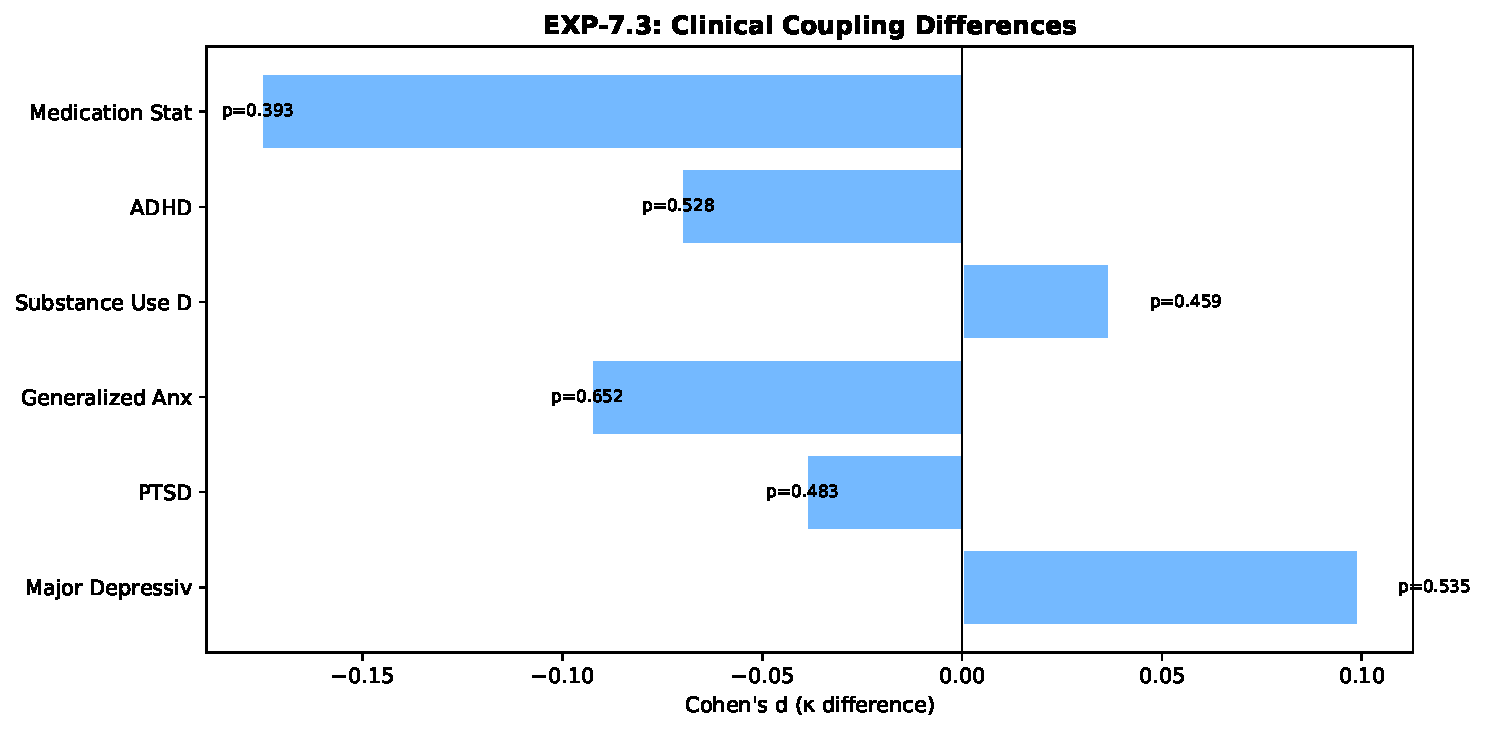
\includegraphics[width=0.85\textwidth]{pictures/chSynthesis/fig_3class_clinical_coupling.pdf}
    \caption{Clinical coupling differences at three-class. Cohen's $d$ for six clinical variables. No diagnosis produces a significant $\kappa$ difference (all $p > 0.39$), replicating the four-class result.}
    \label{fig:ch7_3class_clinical}
\end{figure}

\subsection{Condition-Conditioned Coupling Structure at Three-Class}

The Frobenius norm test for pattern-level Negative--Pleasant differences in the coupling matrix produces $p = 0.376$, and zero of $14$ individual cells reach Bonferroni significance (Figure~\ref{fig:ch7_3class_condition}). The coupling structure does not measurably reorganize between emotional conditions at three-class resolution.

This contrasts with the four-class result, where the Cute--Erotic within-valence contrast produces a significant $\kappa$ difference ($\Delta\kappa = +0.031$, $p = 0.025$) concentrated in temporal-structure metrics. The between-valence Negative--Pleasant contrast at three-class does not modulate coupling; the within-valence Cute--Erotic contrast at four-class does. This reveals that coupling reorganization requires finer-grained affective distinctions than the coarse valence grouping provides---the same content that the arousal hierarchy in Chapter~\ref{chap:arspi_net} identified as the reservoir's most sensitive discrimination axis.

\begin{figure}[H]
    \centering
    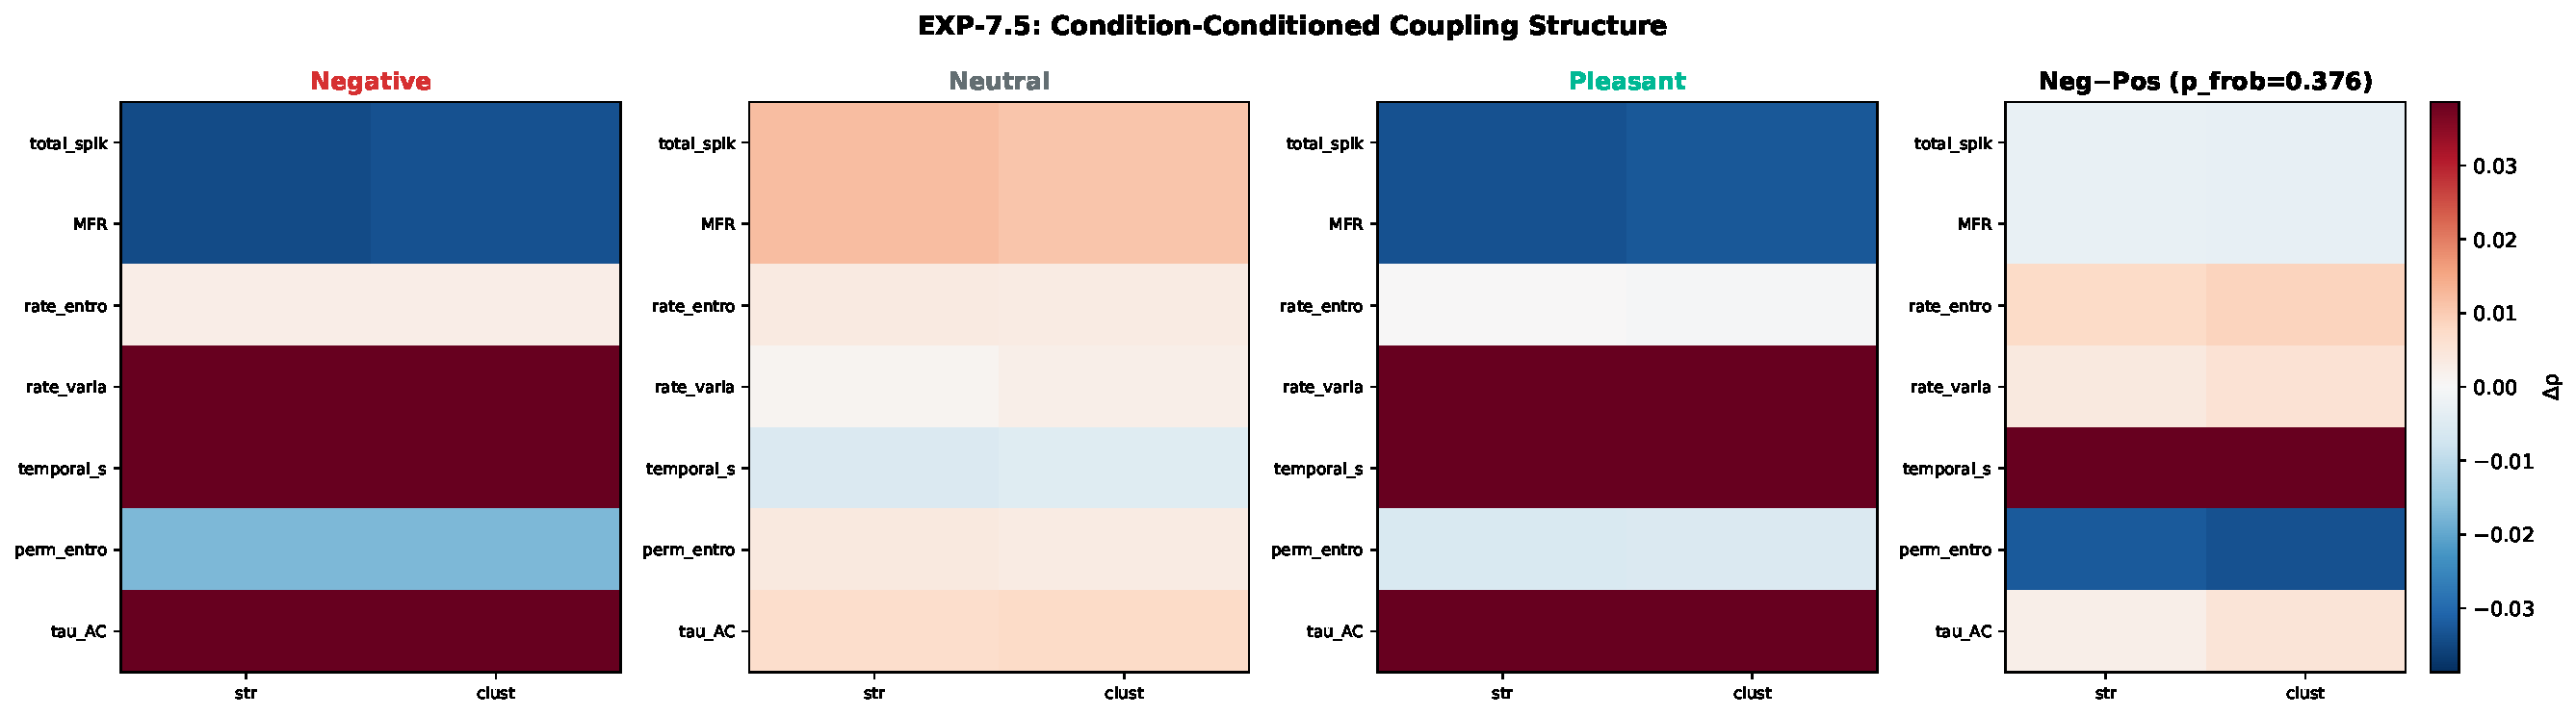
\includegraphics[width=\textwidth]{pictures/chSynthesis/fig_3class_condition_coupling.pdf}
    \caption{Condition-conditioned coupling structure at three-class. Left three panels: per-condition coupling matrices. Right: Negative$-$Pleasant difference matrix with Frobenius norm test ($p = 0.376$). The coupling structure does not reorganize between Negative and Pleasant. At four-class, the Cute--Erotic contrast produces $p = 0.025$---coupling reorganization requires within-valence resolution.}
    \label{fig:ch7_3class_condition}
\end{figure}

\subsection{Augmentation Ablation at Three-Class}

Combined T+D features ($306$ dimensions) do not consistently outperform T-only ($68$d) or D-only ($238$d) on any clinical detection task at three-class (Figure~\ref{fig:ch7_3class_augmentation}). The four-class ADHD finding (D-only AUC $= 0.622$, with $\kappa$ augmentation $p = 0.001$) does not replicate at three-class, where all accuracies are near chance ($43$--$53\%$). The ADHD coupling--augmentation signal appears to require the finer affective resolution of the four-class design.

\begin{figure}[H]
    \centering
    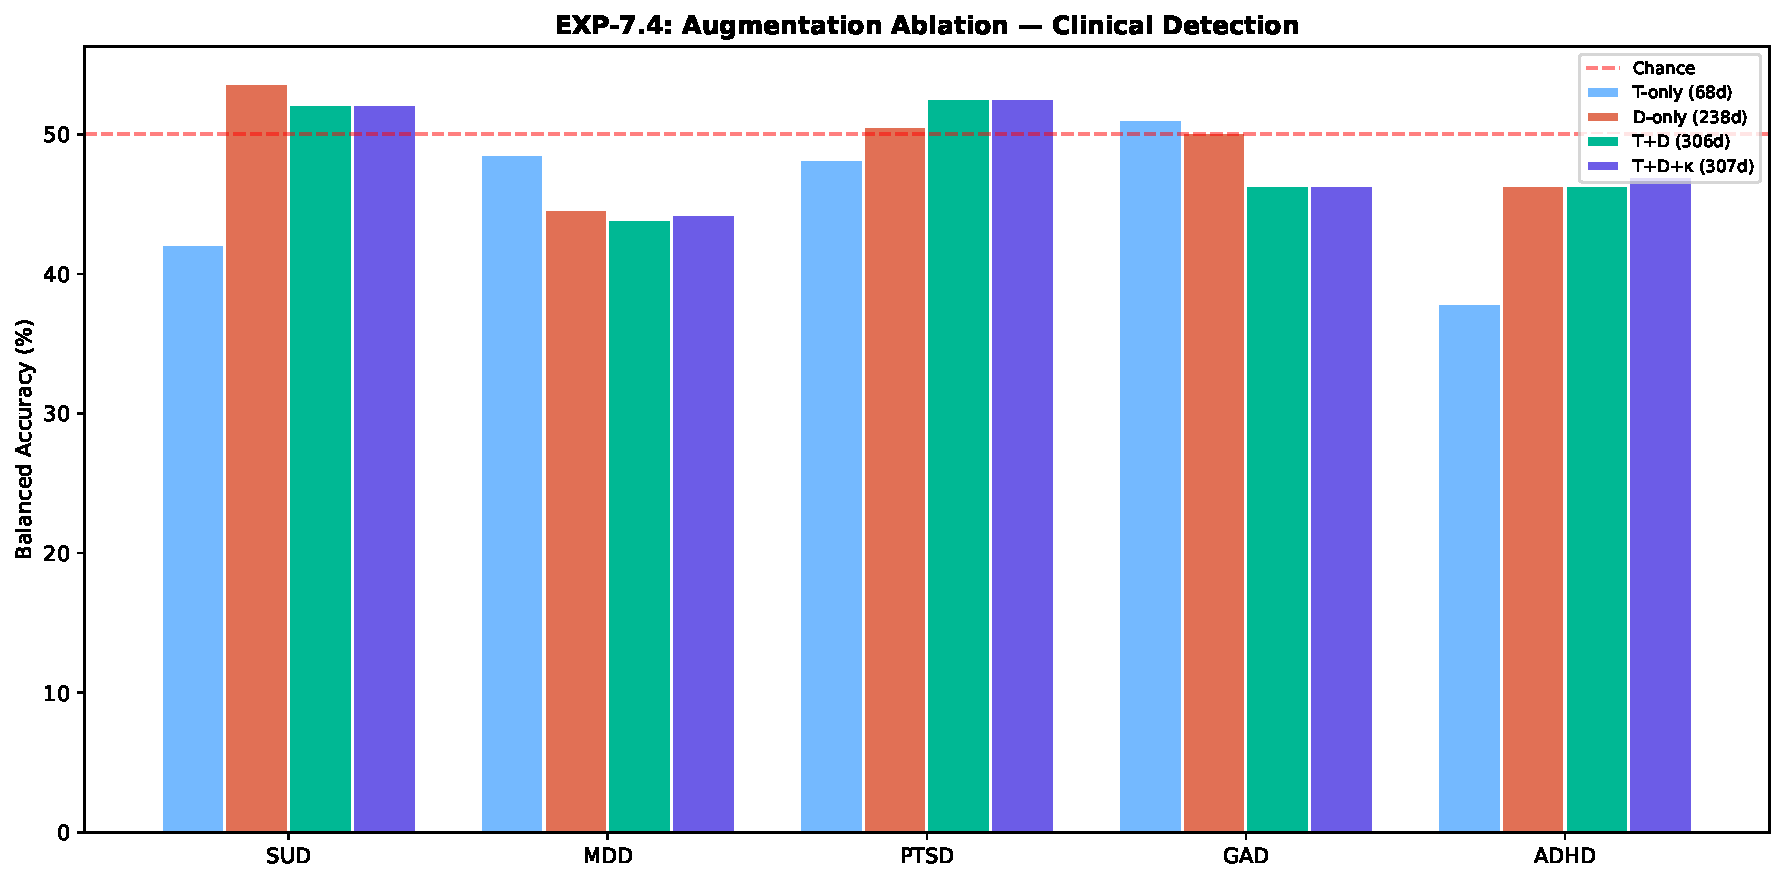
\includegraphics[width=0.85\textwidth]{pictures/chSynthesis/fig_3class_augmentation.pdf}
    \caption{Augmentation ablation at three-class. Balanced accuracy for T-only, D-only, T+D, and T+D+$\kappa$ across five disorders. No combination consistently outperforms the best individual family, replicating the four-class finding that the descriptor families are organizationally related but not discriminatively complementary.}
    \label{fig:ch7_3class_augmentation}
\end{figure}

\subsection{Cross-Granularity Summary}

Table~\ref{tab:ch7_cross_granularity} summarizes the coupling results across both granularities.

\begin{table}[H]
\centering
\caption{Cross-granularity comparison of structure-function coupling results.}
\label{tab:ch7_cross_granularity}
\small
\begin{tabular}{lcc}
\hline
\textbf{Property} & \textbf{3-class} & \textbf{4-class} \\
\hline
Mean $\kappa$ & $0.221$ & $0.199$ \\
Permutation $p$ & $0.000$ & $5.0 \times 10^{-113}$ \\
Coupling direction & Mixed ($6/14$ negative) & Uniform (all negative) \\
Subject variance & $40.3\%$ & $29.2\%$ \\
Condition variance & $0.7\%$ ($p = 0.101$) & $0.6\%$ ($p = 0.133$) \\
Residual variance & $59.0\%$ & $70.1\%$ \\
Clinical $\kappa$ differences & None significant & None significant \\
Condition coupling reorganization & Not significant ($p = 0.376$) & Cute--Erotic $p = 0.025$ \\
Augmentation gain & None & ADHD D-only $0.622$; $\kappa$ $p = 0.001$ \\
\hline
\end{tabular}
\end{table}

Coupling is robust across both granularities: it exists, it is observation-specific, and it does not carry independent clinical discriminative power. The granularity-dependent findings are the coupling direction (mixed at three-class, uniformly negative at four-class), the condition-conditioned reorganization (requires within-valence resolution), and the ADHD augmentation signal (requires four-class resolution). These regime differences are consistent with the granularity-dependent findings in Chapter~\ref{chap:arspi_net}: the four-class resolution accesses finer-grained affective structure that the three-class grouping collapses.


\section{Chapter Synthesis}
\label{sec:ch7_synthesis}

Ten experiments across two granularities converted the relationship between ARSPI-Net's temporal and spatial characterization axes from a hypothesis into a quantified empirical result.

Coupling exists at both granularities ($p < 10^{-3}$) with mean $\kappa \approx 0.2$. The coupling direction shifts from uniformly negative at four-class to mixed at three-class, indicating that the sign structure of dynamical--topological alignment is sensitive to the affective resolution of the driving input. Subject variance accounts for $29$--$40\%$ of coupling variance, with the remainder dominated by observation-specific residual---coupling is not trait-like but rather a property of each individual measurement instance.

No clinical group differs in coupling strength at either granularity. The temporal and spatial axes each carry diagnosis-associated signals independently (Chapter~\ref{chap:arspi_net}: SUD $p = 0.0004$; Chapter~\ref{chap:dynamics}: per-channel SUD $53.6\%$ in ablation), but their alignment does not carry the same signal. Combining the two descriptor families never improves classification beyond the better individual family. The coupling layer is an organizational descriptor of the architecture's internal structure, not an additive discriminative feature.

Two coupling properties are uniquely accessible at four-class resolution: the Cute--Erotic coupling reorganization ($p = 0.025$) concentrated in temporal-structure metrics, and the ADHD $\kappa$-augmentation signal ($p = 0.001$). Both require within-valence affective resolution that the three-class design collapses. These findings converge with the regime boundary identified in Chapter~\ref{chap:arspi_net}: the four-class resolution accesses finer-grained structure in the coupling space, just as it reveals the arousal hierarchy and PTSD threat-specificity interaction in the classification space.

\subsection{The Three-Layer Architecture: An Integrated View}

The complete experimental program across Chapters~\ref{chap:arspi_net}--\ref{chap:synthesis} supports the following characterization of ARSPI-Net as an intrinsically interpretable measurement framework. The architecture reveals three operationally distinct response layers in affective EEG, each producing named, inspectable quantities that a clinician can evaluate without post-hoc explanation methods:
\begin{enumerate}
    \item The \textbf{discriminative embedding layer} (BSC$_6 \to$ PCA-64) carries the richest linearly separable emotion signal within the ARSPI-Net feature families ($59.4\%$ uncentered, $78.8\%$ centered). Per-subject centering reveals $+13$ to $+21$~pp of buried accuracy across all seven tested representations, including EEGNet ($72.0\% \to 89.1\%$). The centering discovery---enabled by ARSPI-Net's geometric transparency---applies to every model in the comparison. After centering, ARSPI-Net matches trained GRU ($78.4\%$) with zero trainable recurrent parameters while providing a fully traceable signal chain.
    \item The \textbf{dynamical response layer} (seven named per-channel trajectory metrics) is condition-sensitive ($7/7$ metrics significant) with the temporal-structure family carrying $2.4\times$ larger effects. Each descriptor has a physical unit and a direct mapping to the input ERP (Chapter~\ref{chap:dynamics}). Subjects organize along a continuous excitability--persistence axis that is condition-modulated but diagnostically independent. The strongest clinical sensitivity in this layer appears for SUD and PTSD, accessible through per-channel spatial resolution.
    \item The \textbf{topology/coupling layer} (graph-topological descriptors and electrode-wise coupling $\kappa$) carries the strongest clinical signals at the graph level (SUD $p = 0.0004$, GAD degree heterogeneity $p = 0.032$) and reveals within-valence coupling reorganization at four-class resolution. Coupling $\kappa$ provides a systems-level interpretability metric: it quantifies whether temporal and spatial characterizations agree at each electrode, producing a per-channel consistency measure that a clinician can inspect directly.
\end{enumerate}
These layers are not interchangeable: the layer ablation in Chapter~\ref{chap:arspi_net} demonstrates that different clinical disorders are most detectable in different layers---dynamics for SUD and PTSD, topology for GAD, coupling for ADHD. This layer-specific clinical interpretability is the dissertation's most distinctive contribution: it provides clinicians with not just a prediction but a structured explanation of \emph{which representational layer} carries the disorder-relevant signal, \emph{which named descriptors} within that layer are atypical, and \emph{how} the patient's temporal--spatial organization compares to the normative population. No black-box architecture---however accurate---can provide this.

\subsection{Level~4 Interpretability Validation: Prototype Clinical Profiling and Cross-Scale Consistency}
\label{sec:ch7_level4}

The coupling analysis established that temporal dynamics and spatial topology are significantly correlated ($\kappa = 0.22$, permutation $p < 0.001$) and that the coupling is observation-specific rather than trait-like. This subsection extends the systems-level interpretability analysis---the fourth and final level of the taxonomy defined in Section~\ref{sec:interp_taxonomy}---through prototype-based clinical profiling.

The $15$ prototypes learned by the interpretable readout (Chapter~\ref{chap:arspi_net}, Section~\ref{sec:interpretable_readout}) assign each observation to a characteristic affective ERP template. Per-subject prototype consistency---the proportion of a subject's three condition observations assigned to the same prototype---averages $\bar{c} = 0.48$, indicating that prototype assignments are condition-dependent rather than subject-fixed. This is the expected behavior: the prototypes capture condition-related response patterns, not stable individual traits.

The prototype transition structure between conditions reveals the affective geometry of the representation. Across the $211$ subjects, the proportion assigned to the same prototype for Negative and Pleasant ($28\%$) is lower than for Negative and Neutral ($35\%$) or Pleasant and Neutral ($33\%$), consistent with the valence contrast between Negative and Pleasant producing more distinct reservoir-transformed representations than either shares with the low-arousal Neutral condition.

Each prototype carries a distinct ERP profile. Among the Neutral-dominant prototypes, Prototype~9 ($93\%$ purity, $n = 27$) and Prototype~5 ($74\%$ purity, $n = 90$) differ in their P300 amplitudes, indicating that Neutral-classified ERPs are further organized into subtypes that the prototype layer exposes. This subtype structure is inaccessible from a flat classifier output.

Mapping the clinical metadata ($211$ subjects, $15$ binary diagnostic variables) onto the dominant prototype assignments reveals diagnostically heterogeneous prototype profiles. Three examples illustrate the clinical structure:
\begin{itemize}
    \item \textbf{Prototype~4} (Negative-dominant, $n = 5$): Persistent Depressive Disorder prevalence of $80\%$ versus $37\%$ in the full cohort ($+43$~pp), PTSD $60\%$ versus $40\%$ ($+20$~pp), MDD Recurrent $80\%$ versus $57\%$ ($+23$~pp). This prototype captures a chronic, comorbid depressive profile with trauma exposure.
    \item \textbf{Prototype~8} (Neutral-dominant, $n = 27$): GAD prevalence of $46\%$ versus $29\%$ ($+17$~pp), with below-population PTSD ($27\%$ vs.\ $40\%$, $-13$~pp) and below-population eating disorders ($23\%$ vs.\ $33\%$, $-10$~pp). This prototype captures an anxiety-predominant profile without trauma or eating pathology.
    \item \textbf{Prototype~13} (Pleasant-dominant, $n = 12$): MDD prevalence of $91\%$ versus $69\%$ ($+22$~pp), with below-population PTSD ($18\%$ vs.\ $40\%$, $-22$~pp) and below-population GAD ($9\%$ vs.\ $29\%$, $-20$~pp). This prototype captures a unipolar depressive profile without comorbid anxiety or trauma.
\end{itemize}
No individual chi-squared test for diagnosis$\times$prototype-class association reaches $p < 0.05$ (all $p > 0.07$, Cram\'{e}r's $V < 0.16$), consistent with the small per-prototype sample sizes ($n = 5$--$40$). These profiles are therefore exploratory and hypothesis-generating, consistent with Rule~11 (Section~\ref{sec:ch5_scope}). The clinical heterogeneity across prototypes---even within the same condition class---demonstrates that the prototype layer exposes patient subgroups whose ERP response organization differs in diagnostically structured ways. A clinician examining the prototype assignment receives not only a condition classification but a pointer to a clinical subtype whose diagnostic composition can be characterized.

Level~4 interpretability is achieved when the systems-level analysis provides information about neural organization that neither temporal nor spatial characterization alone can access. The combination of condition assignment (which prototype), purity estimate (how confident), transition structure (how conditions relate), and ERP profile (what the prototype's temporal signature looks like) produces a multi-dimensional patient characterization that a clinician can evaluate directly. The coupling metric $\kappa$ provides the additional systems-level test of whether the temporal and spatial characterizations agree, completing the four-level interpretability chain that begins with temporal traceability (Chapter~\ref{chap:embeddings}), passes through geometric transparency (Chapter~\ref{chap:arspi_net}) and dynamical characterization (Chapter~\ref{chap:dynamics}), and concludes here with systems-level correspondence.

No existing EEG analysis system provides Level~4 interpretability. ProtoPMed-EEG \cite{barnett_protopmed_2024} provides prototype matching but does not measure cross-scale coupling. NeuCube \cite{kasabov_neucube_2014} provides connectivity analysis but does not formalize the coupling between temporal descriptors and spatial topology as a quantitative metric. EEGNet with SHAP provides no systems-level analysis. The coupling analysis and prototype clinical profiling developed in this chapter represent, to our knowledge, the first demonstration of systems-level interpretability in a neuromorphic EEG architecture, and the first evidence that the multi-layer decomposition produces clinically differentiated prototype subtypes within each condition class.

\subsection{Scope and Future Directions}

The present work characterizes coupling on category-level trial-averaged EEG from a transdiagnostic community sample using theta-band tPLV and two primary topological metrics. Single-trial processing, which would exploit trial-to-trial coupling variability, is a productive extension. Connectivity robustness across frequency bands (alpha, beta, broadband Pearson) and graph-construction thresholds would strengthen the generalization claims. The ADHD coupling--augmentation convergence identified across Experiments~7.4 and~7.5 motivates a targeted study with matched ADHD and control groups. The $\tau_{AC}$ cell-level effects at $d_z \approx 0.16$ require approximately $N = 480$ for Bonferroni-corrected significance, providing a concrete sample-size target for replication. Dimensional clinical measures (symptom severity scales rather than binary diagnoses) may reveal coupling--symptom associations that categorical comparisons miss.